% =====================================================================
%  Capitolo 10 — Il feedback: come darlo, come raccoglierlo e come
%  spacchettarlo; il versioning tracker e il documento di playtest
%  (Game Design, primo anno)
%  Fonte: trascrizione della lezione GD10 (Game Design, primo anno),
%  stesso docente del capitolo 9 (compendium, vision, Theory of Planned
%  Behavior), di cui la lezione è la diretta prosecuzione.
%  Contenuti, nell'ordine della lezione: il task su compendium e vision
%  di Metroid Dread; la legenda della formattazione (domanda di
%  Francesco); il disclaimer sui task di design consegnati (il battle
%  pass, i casi limite, le nuove parole chiave); la premessa sulla
%  severità dei feedback; gli assunti di base (l'umano dall'altra parte,
%  le soft skill, il feedback costruttivo); le regole del feedback
%  (costruttivo, neutrale, sincero, risolutivo, senza giudizio) e la
%  tecnica del sandwich; chiari, precisi, analitici; le pillole
%  aggiuntive (veritieri, teamwork, nomenclature e framing, linguaggio
%  corporeo); il task per la lezione successiva (le concept art di
%  "Zoe") e il fiero; dopo la pausa, raccogliere i feedback (test,
%  chiedere, collezionare), i survey e la scala di Likert, lo
%  spacchettamento dei feedback (l'esempio di God of War), i feedback
%  dai competitor, la curva normale dell'utenza e i consigli finali;
%  nella "lezione jolly", il versioning tracker e il documento di
%  playtest; la chiusura sulla documentazione pratica.
%  Integrazioni da "The Art of Game Design" (Jesse Schell) e da "21st
%  Century Game Design" (Bateman e Boon), segnalate come
%  approfondimenti.
%
%  Pacchetti richiesti nel preambolo del libro (già presenti nel
%  main.tex): \usepackage{booktabs}, \usepackage{amsmath},
%  \usepackage{tikz} con
%    \usetikzlibrary{shapes.geometric,shapes.symbols,shapes.misc,
%      arrows.meta,positioning,calc,fit}
%  (le librerie vanno caricate nel preambolo, non nel capitolo).
%  Tutte le etichette di questo capitolo hanno il prefisso "gd10:"
%  (gd10:sec:..., gd10:fig:..., gd10:tab:...) e tutti gli stili TikZ il
%  prefisso "gd10", per non collidere con gli altri capitoli.
%
%  Nota sulla fonte: la trascrizione automatica è buona nella parte
%  teorica. Come nel capitolo 9, l'inizio della registrazione e la
%  pausa sono stati trascritti come un'unica frase ripetuta in loop
%  ("Grazie a tutti per l'attenzione... Qual è la risposta che ci può
%  essere?"): sono artefatti, omessi. Molti nomi propri (di giochi,
%  persone, strumenti) sono storpiati: dove il riferimento è
%  ricostruibile con certezza lo si riporta nella forma corretta; dove
%  non lo è, lo si segnala in nota invece di indovinare. Le slide non
%  erano state caricate durante la prima parte della lezione: figure e
%  tabelle sono ricostruzioni schematiche di ciò che il docente
%  descrive, non le slide originali.
% =====================================================================

\chapter[Dare, raccogliere e tracciare il feedback]{Il feedback: come
darlo, come raccoglierlo, e i documenti che lo tracciano}
\label{gd10:cap:feedback}

La lezione riprende il filo del capitolo precedente
(capitolo~\ref{gd9:cap:agency-visione}): i task su compendium e vision sono
appena stati assegnati, e i feedback sui task di design (i \emph{pain point}
dei giochi di carte collezionabili) sono appena arrivati agli studenti.
``Dato che ormai li avete ricevuti'', dice il docente, ``sembra doveroso
iniziare a parlarne in maniera più approfondita''. Quella di oggi è quindi
la \textbf{lezione sui feedback}: come si danno, come si ricevono, come si
raccolgono dai giocatori e come si leggono. La lezione finisce in anticipo,
e il tempo avanzato viene speso in una ``lezione jolly'' su due documenti
legati al playtest. La struttura, e quindi quella del capitolo, è questa:
\begin{enumerate}
  \item le questioni in apertura: il task su \textbf{compendium e vision di
        \emph{Metroid Dread}}, la \textbf{legenda della formattazione} e un
        disclaimer sui task di design consegnati, cioè l'obbligo di
        \textbf{scendere nel dettaglio}
        (sezioni~\ref{gd10:sec:apertura}--\ref{gd10:sec:dettaglio});
  \item come \textbf{dare} un feedback: la premessa sulla severità, gli
        assunti di base, le regole del feedback costruttivo, la tecnica
        del sandwich (che non funziona), l'essere chiari, precisi e
        analitici, e alcune pillole aggiuntive
        (sezioni~\ref{gd10:sec:premessa}--\ref{gd10:sec:pillole});
  \item il \textbf{task} per la lezione successiva, con le concept art di
        un ipotetico gioco di zombie, e l'emozione del \textbf{fiero}
        (sezione~\ref{gd10:sec:task-zoe});
  \item dopo la pausa, come \textbf{raccogliere} i feedback: i test, il
        target audience, i dati, i \textbf{survey} e la scala di Likert
        (sezioni~\ref{gd10:sec:raccogliere} e~\ref{gd10:sec:survey});
  \item come \textbf{spacchettare} i feedback, con l'esempio del primo
        \emph{God of War}, e come leggerli nei canali dei competitor
        (sezioni~\ref{gd10:sec:spacchettare}
        e~\ref{gd10:sec:competitor});
  \item la \textbf{curva normale} dell'utenza e i consigli finali:
        problemi e non soluzioni, difendere la visione, \emph{data
        informed} e non \emph{data driven}
        (sezione~\ref{gd10:sec:gaussiana});
  \item la lezione jolly: il \textbf{versioning tracker} e il
        \textbf{documento di playtest}
        (sezioni~\ref{gd10:sec:jolly}--\ref{gd10:sec:playtest-doc});
  \item la chiusura, sulla documentazione pratica e sul lavorare entro dei
        limiti (sezione~\ref{gd10:sec:chiusura}).
\end{enumerate}

% ---------------------------------------------------------------------
\section{In apertura: il task su compendium e vision}
\label{gd10:sec:apertura}

\subsection{Documentare, finché non avrete di meglio da fare}

Fatte le presenze (la lezione è in presenza per tutti, nessuno da casa), il
docente ricollega la giornata alla precedente: la documentazione è
particolarmente importante, ``finché non lo diventerà più, o meglio, finché
avrete qualcosa di più rilevante da fare'', senza però mai dimenticarla,
perché è \textbf{alla base del progetto}. Prima della lezione vera e propria
annuncia \textbf{tre argomenti} su cui espandere: il task in scadenza, un
eventuale ritorno sugli strumenti di comunicazione e i task appena
commentati.

\subsection{Ricordatemi i task}

Il primo punto è il task da consegnare ``per venerdì prossimo, cioè per
questo venerdì'', assegnato il venerdì precedente: il \textbf{compendium} e
la \textbf{vision} di \emph{Metroid Dread}. Il docente lo aveva ricordato
``proprio in calcio d'angolo'', alla fine della lezione, e ne approfitta per
fissare una regola: \textbf{se durante la lezione dice ``poi vi do il task'',
gli studenti glielo devono ricordare}. ``Non fate i furbi'': se il docente se
ne ricorda un giorno dopo, quel giorno gli studenti lo hanno perso. Quindi
non bisogna esitare a fermarlo.

\subsection{Il compendium di Metroid Dread}

Qualcuno aveva chiesto, dopo la lezione, come riempire un compendium senza
avere i documenti del gioco. La risposta: il compendium
(sezione~\ref{gd9:sec:compendium}) \textbf{resterà relativamente vuoto}, ed
è normale. Ciò che interessa al docente è che:
\begin{itemize}
  \item lo si \textbf{divida in categorie}, cioè in \textbf{dipartimenti}:
        non tutti quelli immaginabili, ma i \textbf{dipartimenti
        principali} coinvolti;
  \item si inizi a pensare a \textbf{che cosa potrebbe esservi presentato}
        su questo progetto;
  \item ci siano gli \textbf{status} (anche solo potenziali) della
        documentazione, \textbf{con annessa legenda};
  \item valga sempre la regola: \textbf{funzione maggiore di forma}.
\end{itemize}
Questa prima parte è relativamente semplice, anche perché almeno un link lo
si ha di sicuro: quello alla vision che si deve scrivere.

\subsection{La vision di Metroid Dread}

La vision (sezione~\ref{gd9:sec:vision}) deve invece contenere \textbf{tutte
le informazioni} viste a lezione: principalmente i \textbf{must do}, i
\textbf{must not}, i \textbf{nice to have}, gli \textbf{unique selling point}
e soprattutto i \textbf{temi}, cioè i pilastri;\footnote{Nella trascrizione
``MassDu, MassNot, Nice2Ev, i Mixed Endpoint e sicuramente temi cluster''.
Le prime tre voci sono chiaramente \emph{must do}, \emph{must not} e
\emph{nice to have}; ``Mixed Endpoint'' è quasi certamente una storpiatura di
\emph{unique selling point}, che con le altre tre voci compone la parte di
design della vision (tabella~\ref{gd9:tab:vision}); ``temi cluster'' sembra
riferirsi ai temi, cioè ai pilastri.} e poi le \textbf{prime emotions} e i
\textbf{prime moods}, che ``ci devono essere''. Narrativa, setting e target
audience si possono invece \textbf{tralasciare} per questa volta, perché
richiedono una parte di pre-produzione che gli studenti non hanno.

Ciò che interessa al docente è l'\textbf{attenzione} a che cosa inserire
nella vision e a come inserirlo, in particolare per i \textbf{pilastri}.
\begin{itemize}
  \item In una produzione reale i pilastri si fissano \textbf{a priori}.
  \item Qui li si fa \textbf{a posteriori}: li si va a \textbf{estrarre dal
        gameplay}, giocando il gioco o guardandolo giocare.
\end{itemize}
E la regola del tre vale per tutto: \textbf{tre prime moods, tre prime
emotions, tre pilastri e (al massimo) tre USP}.\footnote{Nella trascrizione
``tre prime mood, tre premie morton, tre pilastri e tre universali
importanti''; gli ``universali'' sono quasi certamente gli \emph{unique
selling point}, per i quali la regola, vista nel capitolo precedente, è
``al massimo tre''.}

\paragraph{Non fate macerare i dubbi.} ``Domande? Tutto chiaro?'' Il
docente insiste: i dubbi non vanno tenuti per sé, ``non facciamoli
macerare''. Parlandone, di solito non solo si risolvono, ma emergono altre
cose interessanti o altri agganci utili.

\subsection{Gli altri due punti}

Il secondo punto, se ci fosse stato tempo, era tornare sulla
\textbf{comunicazione}: esempi, strumenti da usare, come sfruttare tutto ciò
che si ha a disposizione. ``Ci sono mille modi diversi''; ma si potrebbe
espandere su quello che mancava, cioè le sezioni dei core elements su
\textbf{obiettivo}, \textbf{regole}, \textbf{risorse} e
\textbf{interazioni} (capitolo~\ref{cap:che-cos-e-un-gioco}). ``Non è
proprio rilevante, non è necessario'', ma se è utile lo si può prendere. Il
terzo punto sono i \textbf{task consegnati e commentati}
(sezione~\ref{gd10:sec:dettaglio}).

% ---------------------------------------------------------------------
\section{Serve una legenda della formattazione?}
\label{gd10:sec:legenda}

Prima di passare ai task, Francesco pone una domanda sulla documentazione:
\textbf{quanto è giusto inserire una legenda} che spieghi gli strumenti di
formattazione che si usano (colori, grassetti, evidenziature)? È utile,
o ``copre spazio e basta''?

\paragraph{Dipende da quanto siete chiari.} La risposta è: dipende, prima di
tutto, da \textbf{quanto è immediatamente comprensibile} per il lettore il
codice che si usa. Se il rosso si usa solo per i nemici o per gli ostacoli
di gioco (``dico un esempio a caso''), quanto è evidente?

\paragraph{Dipende da quanti elementi usate.} Se ci sono \textbf{acronimi},
nomi specifici che si legano ad altri elementi del documento (come nel caso
degli \textbf{status} del compendium), la legenda diventa
\textbf{necessaria}. Se si usa un \textbf{enorme numero} di strumenti
(corsivo, grassetto, sottolineato, evidenziatura, $N$ colori diversi), allora
potrebbe esserlo. Non c'è un numero preciso.

\paragraph{Una legenda della formattazione a monte?} Se lo stile fosse
davvero \textbf{codificato} (``usiamo sempre il rosso per una data cosa''),
si potrebbe pensare a un \textbf{documento a parte}, una legenda a monte che
spieghi tutto lo stile di documentazione: ``un po' un production dictionary
per la formattazione'' (sezione~\ref{sec:production-dictionary}). Ma il
docente precisa due volte di \textbf{non averlo mai visto}, e che un
documento del genere assume che \textbf{tutti usino lo stesso stile}, il che
non è sempre vero. Ogni designer ha il proprio stile di documentazione: anche
quando ci sono limiti stringenti (lo si vedrà con il \textbf{GDD}, in cui
alcuni paragrafi devono esserci per forza), ``ho sempre visto grande margine
di differenze creative o stili di formattazione''.

\paragraph{L'obiettivo è non renderla necessaria.} Una legenda può essere
utile; l'obiettivo, però, è \textbf{scrivere in modo che non serva}. L'unico
caso in cui il docente la ritiene generalmente utile è quello dei documenti
\textbf{veramente complessi}, grossi e con tante variabili: i
\textbf{documenti di bilanciamento}, gli Excel enormi, in cui ``il primo
foglio è generalmente atto a spiegare questa roba qua'', con una legenda
sempre visibile immediatamente.

% ---------------------------------------------------------------------
\section{Il disclaimer sui task: il design va descritto nel dettaglio}
\label{gd10:sec:dettaglio}

\subsection{Un design amputato}

Sui task consegnati, il docente fa un disclaimer ``di venti secondi'' (che
dura parecchio di più). Il task era un \textbf{primo tentativo di analisi,
con conseguenti soluzioni di design} proposte dagli studenti. Il docente non
si aspettava soluzioni \emph{groundbreaking} o modi di fare design
esagerati; e nella parte di \textbf{analisi} ci sono spunti più o meno
corretti. Ma la parte di \textbf{design}, e questo vale per tutti,
\textbf{mancava di pezzi specifici}: ``come se fosse proprio amputata in una
parte''. Non è un problema, adesso: si vedrà come si fa.

\paragraph{Documentare qualcosa che non esiste.} Quando si documenta una
soluzione che non esiste ancora (perché la si è creata, o perché la si
prende da altrove), bisogna essere \textbf{specifici, puntuali, precisi}: è
la solita questione della documentazione. E il modo migliore per farlo è
dare \textbf{esempi concreti}, visibili, magari in \textbf{tabella}.

\subsection{L'esempio del battle pass}

Alcuni studenti avevano proposto un nuovo sistema di progressione o di
\emph{reward} appoggiato a esempi noti: i \emph{daily reward} legati al
login, o un \textbf{battle pass}. Anche nella versione più macroscopica, va
specificato:
\begin{itemize}
  \item da \textbf{quanti elementi} è composto, cioè da quanti
        \textbf{livelli}, almeno indicativamente;
  \item \textbf{quanta esperienza} serve per un livello, magari non
        esattamente, ma almeno se è \textbf{la stessa} per ogni livello o se
        \textbf{cresce};
  \item \textbf{che cosa succede quando il battle pass viene finito}.
\end{itemize}

\paragraph{I casi limite.} Molte soluzioni descrivevano solo \textbf{il caso
migliore}, quello in cui tutto va come previsto. ``Ed è questo che manca a
molti designer'': bisogna pensare anche ai \textbf{casi limite}. Il giocatore
che finisce tutto il battle pass, poi che fa? Può continuare a
\emph{grindare} per una ricompensa, oppure no, non succede nulla: va bene
tutto, ma \textbf{c'è una scelta da fare, e va esplicitata}. Sono gli stessi
casi limite visti nella ricerca, nel brainstorming e nella generazione delle
idee (capitolo~\ref{cap:brainstorming-flowchart}).

\subsection{Nuove UI e nuove carte}

Lo stesso vale per qualsiasi nuova \textbf{UI}: che cosa contiene, come ci si
interagisce. E per una \textbf{nuova carta}: qual è l'effetto? Nel caso dei
giochi di carte del task non è particolarmente interessante avere il numero
esatto di attacco e difesa, o (per le carte di \emph{Marvel Snap}) il costo
in mana e l'attacco bilanciati. Ma se si inserisce un \textbf{effetto
innovativo} o una \textbf{nuova parola chiave}, quella \textbf{va
spiegata}.

\subsection{Fare design significa trattare tutti i dettagli}

Ci si arriverà piano piano, fino al \textbf{game design document}, che si
vedrà l'anno successivo (``2026, sempre con me, non ora''). Ma va capito
subito che \textbf{fare design significa trattare tutti i dettagli}. È il
motivo per cui il docente è ``così rompipalle'' su alcuni elementi dei task:
essere precisi, non usare a caso tutti gli strumenti, non lasciare spazio
sprecato.

\paragraph{Non un wall of text.} Elencare tutti i dettagli non significa
scrivere un \emph{wall of text}, ma \textbf{mostrarli}: per esempio con i
\textbf{flowchart} appena visti (sezione~\ref{sec:flowchart-usi}), che si
possono usare nella documentazione di design. Si tratta di trovare il modo
migliore per mostrare un sistema nel modo più chiaro possibile \textbf{a
qualcuno che non lo conosce} e che eventualmente lo dovrà
\textbf{implementare}.

\paragraph{I programmatori fanno di testa loro.} Il caso tipico è il
programmatore: ``se non glielo dite, fanno di testa loro''. Ed è ``la
peggior causa possibile'': inseriscono una feature che \textbf{non è la
vostra}, e di cui poi \textbf{siete voi responsabili}.

\paragraph{Il tallone d'Achille.} Spiegare il design nel dettaglio è
``il tallone d'Achille''\footnote{Nella trascrizione ``il pallone da
killer'', presentato dal docente come ``una grande citazione, colta o non
colta, a seconda dei casi''. È quasi certamente il \emph{tallone d'Achille}.}
di molti designer, ed è ciò che \textbf{differenzia una persona competente
da una non competente}.

\paragraph{Il test dell'implementazione.} L'invito finale è a ritornare sulle
proprie soluzioni e chiedersi se sono chiare. Visto che gli studenti hanno
da poco iniziato a programmare, il test è questo: \emph{se dovessi
implementare io questo sistema, avrei tutti gli estremi per scrivere il
codice e inserirlo nel gioco? E un giocatore che lo giocasse avrebbe tutti
gli estremi per farlo? Ho considerato tutte le possibili interazioni?} Non è
esattamente ciò che il task chiedeva, ``però fare design poi significa
questo''.

% ---------------------------------------------------------------------
\section{Una premessa sulla severità}
\label{gd10:sec:premessa}

\subsection{Niente di personale}

Si entra nella lezione sui feedback (``\emph{feedback}, non traducibile in
italiano, purtroppo: che peccato''). Il docente fa subito una premessa che
con le classi precedenti faceva più tardi: va contestualizzata la
\textbf{severità} dei feedback dati e ricevuti, perché non venga
``assorbita'' nel modo sbagliato.
\begin{itemize}
  \item \textbf{Nulla} di ciò che il docente dice o commenta è rivolto
        \textbf{alla persona}.
  \item Tutto ciò che fornisce è \textbf{in funzione della crescita} dello
        studente.
  \item Si può discutere su un certo tipo di severità, ma è
        \textbf{necessaria}, ``ed è per il vostro bene'': l'obiettivo è
        migliorare il lavoro, far raggiungere uno step successivo.
\end{itemize}

\subsection{Il mondo là fuori}

L'obiettivo è \textbf{preparare a un domani} in cui, nel migliore dei casi,
si è già abituati a ricevere un certo tipo di feedback e di commenti, perché
alcuni di questi \textbf{non ricadono esattamente nel feedback costruttivo}:
si potrebbe non avere il privilegio di riceverli in maniera corretta, ``e ve
lo dico per esperienza personale''. In quel caso bisogna aver sviluppato la
\textbf{pelle dura} nel proprio percorso, oppure trovare il modo di
``smarcare'' la cosa, riassestarsi e salvare il proprio posto, la propria
sanità mentale e quella di tutti. Non è esattamente responsabilità del
designer, ma è un problema in cui si potrebbe incorrere.

\paragraph{Non restare attivati.} C'è poi una tendenza, più frequente in
chi è più giovane, a \textbf{restare attivati}: ad assorbire ciò che si
legge o che viene detto come un attacco personale. Cosa che, ripete il
docente, non vuole assolutamente essere il caso.

\subsection{Che cosa si vedrà}

La lezione tratterà come \textbf{dare} ed eventualmente \textbf{raccogliere}
feedback: prima in maniera generica, all'interno dei progetti, come
professionisti; poi nelle \textbf{sessioni di playtest}, momenti più
circoscritti. E c'è un altro beneficio: saper dare feedback aiuta a
\textbf{collaborare}. Finché non si sa parlare correttamente con gli altri,
soprattutto con chi fa un lavoro diverso dal proprio, è difficile, o
rischioso, avere team grossi e sapere come aggiustare il tiro al loro
interno.

\paragraph{Il meme.} La slide di apertura mostra un gatto che porge una rosa
(``questo non è un meme, sono io che vi porgo l'altra guancia''): il gatto è
il docente, dall'altra parte ci sono gli studenti che ricevono i suoi
commenti e le sue mail, ``che sono 230.637''. ``Non è un feedback,
comunque.''

\paragraph{Un precedente.} Gran parte di questi temi era già stata toccata,
da un'altra angolatura, nel seminario sulla cultura del feedback
(capitolo~\ref{cap:z1-feedback}, in particolare le
sezioni~\ref{sec:z1-dare} e~\ref{sec:z1-ricevere}): qui il punto di vista è
quello del designer, nel team e davanti ai giocatori.

% ---------------------------------------------------------------------
\section{Gli assunti di base}
\label{gd10:sec:assunti}

\subsection{Dall'altra parte c'è un umano}

L'assunzione di base nel comunicare, nel lavorare in gruppo e nel far capire
agli altri se hanno fatto bene o male è che \textbf{dall'altra parte c'è un
essere umano}. ``Non so se avete mai provato a controllare se avete un
esoscheletro'': per ora si parla di umani che parlano ad altri umani, ``poi
magari in futuro cambierò le slide''. Quindi serve un certo tipo di
\textbf{empatia}.

\paragraph{Egoless, ma umani.} È vero che il design è \emph{egoless}; ma chi
fa design è un essere umano, e ci saranno spesso momenti in cui si parlerà
in maniera umana. Ci sono contesti lavorativi regolati, come quello dei
feedback, e altri meno regolati, ed è bene così: un grande motivo per
lavorare in questo campo è che le persone tendono ad avere \textbf{molte
cose in comune}, ed è più facile fare \emph{bonding}, stringere amicizie.
Ma resta il fatto che dall'altra parte c'è qualcuno che assorbe ciò che gli
si dice, e viceversa.

\subsection{Le soft skill}

Il secondo assunto, ``la cosa più importante'', poco rilevante al primo anno
ma estremamente importante dal secondo in poi, sono le \textbf{soft skill}.
La slide ne mostra una lista ``non omnicomprensiva'', con quelle
illustrazioni dall'estetica aziendale di cui il docente ha appena scoperto
che esiste un nome (``mi fa morire''):\footnote{Il docente dice ``corporate
qualcosa''. Lo stile di illustrazione piatta, con figure dalle membra
allungate, molto diffuso nella comunicazione aziendale, è comunemente detto
\emph{Corporate Memphis}.}
\begin{itemize}
  \item comunicazione chiara;
  \item capacità di ascolto;
  \item autocontrollo (``la capacità di non uccidere altre persone'');
  \item attitudine positiva;
  \item assertività;
  \item risoluzione dei conflitti;
  \item empatia;
  \item depersonalizzazione;
  \item prendersi le responsabilità;
  \item un pizzico di humor.
\end{itemize}

\paragraph{Nel team ci si compensa.} La lista delle soft skill è enorme, e
non tutti devono essere spiccatamente positivi o avere un grande senso
dell'umorismo: all'interno del team \textbf{ci si compensa}.

\paragraph{La prima discriminante.} Ma questa è, ``purtroppo, per fortuna
anche qui'', \textbf{il primo elemento considerato per essere assunti o
licenziati}. Le persone che vogliono lavorare con qualcuno non lo fanno
principalmente perché è un bravo tecnico o ha estreme skill di design, ma
per le sue \textbf{soft skill}. Le competenze (level design, narrative,
programmazione, game design) ci devono essere; ma la prima discriminante
sono queste, come lo sono per essere mandati a casa: se si alzano le mani su
qualcuno o lo si insulta, la cosa viene punita, con una lettera di richiamo
o con il licenziamento, a seconda dell'azienda.

\paragraph{Con gli altri dipartimenti.} Le soft skill diventeranno
notevolmente più importanti nei \textbf{progetti di gruppo}, soprattutto
quando questi si proietteranno su altri dipartimenti: arte, programmazione,
narrativa. Lì non si parla solo con altri esseri umani, ma con esseri umani
che potenzialmente \textbf{non condividono il proprio linguaggio tecnico}.

\subsection{I feedback sono costruttivi}

Il terzo assunto è che \textbf{i feedback sono costruttivi}. ``Non siamo qui
per dire `il tuo lavoro è una merda'{}'': siamo qui per formulare un feedback
che sia \textbf{recepito in modo chiaro} e che vada a \textbf{migliorare il
lavoro dell'altro}, o il nostro, se il progetto è condiviso.

\subsection{Feedback 101}

Le cose di base (``\emph{basic things to say}'') sono tre.
\begin{description}
  \item[Precisi e rispettosi] In ciò che si dice si è \textbf{precisi e
        netti}. Questo \textbf{non} significa nascondere le cose, o non
        parlare se c'è un problema: è tutto il contrario. Ma nel dirlo si
        è \textbf{rispettosi} del lavoro degli altri, del tempo dedicato, e
        così via. Si è \textbf{onesti}, e dall'altra parte si sa
        \textbf{ascoltare}, con l'umiltà di capire che cosa viene detto. Si è
        \textbf{professionisti} e \textbf{composti}: non lo si dice
        arrabbiandosi o ribaltando il tavolo, ma nemmeno abbracciando il
        collega e dandogli pacche sulla spalla.
  \item[Empatia] Il discorso dell'essere umano. Come metro di misura, si
        cerca di capire \textbf{in che situazione è il collega}: ha delle
        difficoltà? Gli è stato rigettato il task (``nel vostro caso
        ventisette milioni di volte'')? Ha dedicato tanto lavoro e tanto
        impegno, ma ritorna agli stessi problemi? Si cerca il punto critico
        che sta passando. E si \textbf{formula il feedback nella propria
        testa} prima di darlo: se lo dicessero a me, c'è il rischio che
        venga assorbito in modo problematico, o frainteso?
  \item[Coltivare] Tutto questo \textbf{va coltivato}.\footnote{Nella
        trascrizione il titolo del terzo punto è illeggibile (``Riso
        scritto''); il contenuto, che ``incapsula'' i due precedenti, è
        chiaramente la necessità di coltivare queste capacità
        relazionali.} Chi ha già lavorato in team, o vive in un contesto
        con molte persone (una famiglia numerosa e stimolante, una grossa
        cerchia di amici che si vedono spesso), è avvantaggiato, per
        tendenza naturale o per esperienza; ma non c'è nulla che non si
        possa coltivare. Il picco, ``perché poi alla fine questo dovrete
        andare a fare'', è la relazione con gli altri in un contesto
        \textbf{formale}, quello lavorativo.
\end{description}

\paragraph{Iniziate a farci caso.} Diventerà più importante al secondo
anno, ma conviene iniziare subito a pensare a come si parla con i colleghi,
a quanto tempo si passa nei propri gruppi (``gruppi illegali in cui siete
con persone che non ci devono essere, non lo so, dipende da voi''), a come
ci si relaziona agli altri, e a quanto ci si fa caso. È la discriminante
principale per cui le persone vogliono o non vogliono lavorare con qualcuno:
perché si trovano bene, perché possono fare affidamento su di lui se hanno
un problema imprevisto, su ciò che sa fare e su come lo sa fare. Si diventa
\textbf{un ponte} tra sé e gli altri: è l'obiettivo del lavoro di gruppo, ed
è anche la difficoltà dei team grandi ed eterogenei.

% ---------------------------------------------------------------------
\section{Come si compone un feedback}
\label{gd10:sec:comporre}

Fissati gli assunti (``il primo passettino''), si passa a come si compone il
feedback in sé. La tabella~\ref{gd10:tab:regole} riassume le cinque regole;
le si vede una per una.

\begin{table}[htbp]
  \centering
  \caption{Le regole del feedback come presentate a lezione.}
  \label{gd10:tab:regole}
  \small
  \begin{tabular}{@{}p{0.2\textwidth}p{0.72\textwidth}@{}}
    \toprule
    \textbf{Regola} & \textbf{In pratica} \\
    \midrule
    Costruttivo & preciso, chiaro, analitico; informazioni chiare, senza
      giri di parole; il termine specifico, non quello più oscuro \\
    \addlinespace
    Neutrale & segnala gli aspetti negativi \textbf{e} quelli positivi, e
      perché; lo fa in uno stato emotivo neutro \\
    \addlinespace
    Sincero & si assume che tutti siano adulti e professionisti: il
      feedback serve al miglioramento, e lo si riceve in modo neutrale \\
    \addlinespace
    Risolutivo & dopo il problema, una \textbf{soluzione attuabile},
      suggerita e non imposta, con margine di manovra \\
    \addlinespace
    Senza giudizio & niente ``bravissimo'', ``ottimo'', ``fa schifo'';
      attenzione soprattutto con i dipartimenti che non si conoscono \\
    \bottomrule
  \end{tabular}
\end{table}

\subsection{Costruttivo}

Si assume che il feedback sia costruttivo, e quindi valgono le solite regole
della documentazione: deve essere \textbf{preciso, chiaro e analitico}.
L'obiettivo è dare, in modo ancora più asciutto che in un documento,
\textbf{informazioni chiare, senza giri di parole}. Se esiste un
\textbf{termine specifico} per una cosa, si usa quello, e non il termine più
oscuro o l'italiano più arcaico ``per sembrare colti''. ``Dovete essere
capiti: questo è il concetto.''

\paragraph{Una confessione sui feedback del docente.} Riallacciandosi alla
premessa, il docente ammette che \textbf{alcuni} (``non molti, alcuni'') dei
suoi feedback sono \textbf{volutamente manchevoli di informazione}: gli
interessa che lo studente faccia il lavoro extra di capire dove fosse il
problema e quale, tra le mille soluzioni possibili, fosse quella adeguata.
``Non nascondo che anche dal lato mio mi salva del tempo.'' Ma non è
l'ideale: l'ideale è aiutarsi nel modo migliore possibile. Quindi, per tutto
ciò che non è comprensibile o sembra manchevole, \textbf{scrivetegli}: o
darà l'informazione, o dirà che non la può dare, e allora si è in quel caso.

\subsection{Neutrale}

Il feedback \textbf{non sottolinea solo gli aspetti negativi}: può e deve
sottolineare anche quelli \textbf{positivi}, che magari si possono comunque
migliorare. Ce ne si dimentica spesso, per due ragioni.
\begin{enumerate}
  \item \textbf{Fattibilità}: se qualcosa funziona, generalmente lo si lascia
        stare e ci si concentra sul negativo, per portarlo a funzionare.
        ``Squadra che vince non si cambia: si migliora, ma non si cambia.''
        La priorità ce l'hanno le cose che non funzionano.
  \item \textbf{Natura umana}: ``siamo di tendenza bastarda come esseri
        umani'', ed è più facile sottolineare il negativo che il positivo.
\end{enumerate}
Ma, sempre per empatia, gli aspetti positivi \textbf{che non vanno
cambiati} vanno detti, perché chi riceve il feedback potrebbe non dare per
scontato che quella cosa funzioni, e cambiarla, magari in peggio. Quindi:
\textbf{quello che funziona, ditelo; quello che non funziona, ditelo; e dite
perché}.

\paragraph{Uno stato emotivo neutro.} Queste cose vanno dette in uno
\textbf{stato emotivo neutro}, nel modo più umano possibile. Non tutti
sanno tenere al guinzaglio le proprie emozioni, ``però ci sono dei libri''.
Il problema tipico è che il negativo viene detto in modo \textbf{rabbioso,
violento, viscerale}; e, all'opposto, il positivo come se fosse il più
grande capolavoro del mondo. Positivo e negativo vanno \textbf{percepiti
nello stesso modo}: una cosa positiva funziona, va bene, o si migliora in un
certo modo; una cosa negativa non è un problema, va sistemata. Il risultato
è lo stesso: lavorare.

\subsection{Sincero}

La sincerità non è solo esprimere sinceramente che cosa funziona e che cosa
no: è l'assunzione, ``ed è il motivo per cui questa lezione la facciamo a
tutti, e bisognerebbe farla in tutti gli altri corsi'', che \textbf{tutti
siano adulti e professionisti}. In un contesto lavorativo, in cui si deve
migliorare il progetto e trovare i problemi, se si dà un feedback non lo si
dà ``per farti rifare il lavoro perché sono bastardo'', ma perché
l'obiettivo è il \textbf{miglioramento}: personale (nel rapporto
docente-studenti) o del progetto (tra colleghi). Di conseguenza, chi riceve
un feedback si mette nell'ottica di recepirlo \textbf{in modo neutrale},
senza esserne intaccato personalmente. E viceversa.

\subsection{Risolutivo}

Sottolineato il problema (o la cosa che funziona), \textbf{ci deve essere un
dopo}. Manca spesso un pezzo, ed è il motivo per cui molti commenti
\textbf{non sono proprio feedback}: la \textbf{parte risolutiva}. Emerso
l'elemento in questione (la mancanza di un dato, la mancanza di una
reference, nell'esempio del design), \textbf{qual è la soluzione attuabile?}
Come si può migliorare? È ``l'aggancio che spesso manca'', e va dato nel
modo più esplicito possibile.

\paragraph{Suggerire, non imporre.} Con un feedback si deve
\textbf{suggerire una strada}, non imporla: ``attenzione''. Più ampio è il
ventaglio di possibilità che si mostra, meglio è. E dall'altra parte,
tornando alla sincerità tra adulti, ci deve essere la maturità di capire che
è \textbf{un consiglio e non un obbligo}: chi riceve il feedback valuta se
quella strada è giusta, o se può ``rubare un pezzo di idea'' e implementare
qualcos'altro che risolva comunque il problema. Nella soluzione ci deve
essere \textbf{margine di manovra}.

\subsection{Senza giudizio}

Soprattutto quando si danno feedback, si cerca di \textbf{non dare
giudizi}: niente ``bravissimo'', ``ottimo'', ``fa schifo''. Il docente
cerca di farlo sempre nel modo più contenuto possibile, ``anche se siamo
umani''. Il giudizio può funzionare come un pizzico di sale (``\emph{as a
sprinkle}''): sempre per empatia, per \textbf{potenziare il morale}, o per
ridimensionare chi è estremamente egocentrico e ``si monta la testa''. Ma
sono strategie \textbf{veramente al limite}.

\paragraph{Con i dipartimenti che non conoscete.} È molto facile cadere nei
giudizi soprattutto con i dipartimenti di cui si sa poco: non si sa quanto
ci ha messo un animatore a fare quell'animazione, né quanto è facile
cambiarla se gli si suggerisce di farlo in poco tempo. E diventa
estremamente importante \textbf{più si sale nella piramide gerarchica}, ``ve
lo dico per esperienza'': da lì possono scaturire estrema maleducazione o
estrema sottovalutazione del tempo dedicato.

\paragraph{L'errore peggiore dei producer.} ``Visto che abbiamo qui il
nostro invitato speciale, anzi, intruso speciale'' (in aula c'è un
ospite legato alla produzione), il docente nomina il peggior errore che un
producer possa commettere: \textbf{non avere conoscenza del tempo pratico}
che servono le cose, e \textbf{non fidarsi} degli altri all'interno del team.

\subsection{La tecnica del sandwich non funziona}

Spesso viene citata la \textbf{tecnica del sandwich}, o del panino: si
comincia con un feedback positivo, ci si infila dentro ``un kebab a tre euro
di schifo'' (tutte le cose negative, magari caricate nel modo sbagliato) e si
chiude con un altro feedback positivo ``per togliere il sapore di kebab
marcio dalla lingua''.

\textbf{Non funziona.} È esattamente il problema di \emph{no judgment} e di
\emph{neutrality} visto prima: non è feedback costruttivo, non è una tecnica
attuabile. Il feedback deve essere \textbf{chiaro}: non lo si deve
nascondere, seppellire o rendere piacevole da digerire. Se riguarda un
aspetto negativo, e l'aspetto è \textbf{critico}, lo si deve far emergere e
mostrare \textbf{quanto} è critico. Sempre in modo neutrale: ``è meglio una
lista chiara che un pappone panino indigeribile''
(figura~\ref{gd10:fig:sandwich}).

\begin{figure}[htbp]
  \centering
  \begin{tikzpicture}[
      gd10slice/.style={draw, rounded corners=6pt, minimum width=4.6cm,
        minimum height=0.75cm, align=center, font=\small},
      gd10row/.style={draw, minimum width=5.6cm, minimum height=0.62cm,
        align=left, font=\footnotesize, text width=5.3cm},
      gd10ttl/.style={font=\small\bfseries, align=center}]
    % il sandwich
    \node[gd10ttl] at (0,2.15) {Il sandwich (non funziona)};
    \node[gd10slice, fill=gray!10] (top) at (0,1.35) {positivo generico};
    \node[gd10slice, fill=gray!35, minimum height=1.3cm] (mid) at (0,0.25)
      {negativo nascosto, annacquato\\ o caricato male};
    \node[gd10slice, fill=gray!10] (bot) at (0,-0.85) {positivo generico};
    \node[font=\footnotesize, align=center, text width=4.8cm] at (0,-2.15)
      {il punto critico si perde: \\ quanto è grave? che cosa si fa?};
    % la lista
    \node[gd10ttl] at (7.2,2.15) {La lista chiara};
    \node[gd10row] (r1) at (7.2,1.35) {\textbf{Funziona:} X, perché\ldots};
    \node[gd10row, below=0pt of r1] (r2) {\textbf{Non funziona (critico):} Y,
      perché\ldots};
    \node[gd10row, below=0pt of r2] (r3) {\textbf{Proposta:} strade A, B,
      C (a scelta)};
    \node[gd10row, below=0pt of r3] (r4) {\textbf{Non funziona (minore):} Z,
      perché\ldots};
    \node[gd10row, below=0pt of r4] (r5) {\textbf{Proposta:} strada D};
    \node[font=\footnotesize, align=center, text width=5.6cm] at (7.2,-2.15)
      {tono neutro per tutto; il peso di ogni punto è esplicito};
  \end{tikzpicture}
  \caption{La tecnica del sandwich contro una lista chiara: ricostruzione
  schematica del confronto fatto a lezione, non la slide originale.}
  \label{gd10:fig:sandwich}
\end{figure}

% ---------------------------------------------------------------------
\section{Chiari, precisi, analitici}
\label{gd10:sec:cpa}

``Fin qui tutto chiaro, intanto?'' Il docente torna sulle tre qualità del
feedback costruttivo e spiega come ottenerle.

\subsection{Chiari}

Evitare terminologie complesse e termini oscuri \textbf{per il solo motivo
di sentirsi più intelligenti}. Il docente ammette di avere proprio questo
problema: parla spesso in termini complessi e con metafore oscure. Se si ha
questa tendenza, si \textbf{riformula}.
\begin{itemize}
  \item Se qualcosa non viene capito, o si ha il dubbio che l'altro non
        stia capendo, lo si dice in un altro modo.
  \item Non solo lo si deve chiedere: \textbf{l'altro lo deve dire}, se non
        ha capito.
  \item Se non è chiaro, si trova un altro modo, finché \textbf{tutti e due
        non sono soddisfatti}.
  \item Riformulare non significa \textbf{ripetere uno a uno}: dire due
        volte la stessa frase non serve.
\end{itemize}

\subsection{Precisi}

Essere precisi significa \textbf{dare le reference}. Se si fa riferimento a
un titolo o a una soluzione già adottata altrove, si dice \textbf{dove,
esattamente quale}: si mostra il \textbf{link al minuto corretto} di un
gameplay, si fa ``la biblioteca'', si prende un'immagine e la si fa vedere.

\paragraph{Fermarsi a guardare insieme.} Se si discute di una meccanica con
un altro designer e l'altro non ha chiaro di che meccanica o di che gioco si
parli, \textbf{ci si ferma}, si va a vedere e si mostra: ci si prende il
tempo per guardarlo e osservarlo insieme. Quel tempo è
\textbf{necessario}.

\paragraph{Dare il tempo di assorbire.} Per lo stesso motivo, se si dà una
reference (``leggi questo libro'', ``gioca questo gioco''), non ci si aspetta
la risposta pronta il giorno dopo: si dà all'altro il \textbf{tempo per
assorbire} ciò che gli si è dato.

\subsection{Analitici}

Essere analitici significa analizzare le reference date e descrivere le
cose \textbf{oggettivamente}, senza dimenticare l'empatia. Le domande da
farsi sono queste.
\begin{itemize}
  \item \textbf{Quale reazione viene evocata} da ciò che si analizza?
  \item \textbf{Qual era l'obiettivo} di ciò che si sta valutando? È un
        prototipo? E qual è l'obiettivo di quel prototipo? Un prototipo
        probabilmente non sarà esteticamente bello: avrà i cubi, avrà gli
        SFX placeholder. Ma il suo obiettivo era magari testare una
        meccanica di sparo, di salto, una meccanica specifica: ``magari ci
        stiamo concentrando sulla cosa sbagliata''. Questo, peraltro,
        dovrebbe dirlo chi consegna il prototipo.
  \item \textbf{Qual era l'intenzione} di chi l'ha creato?
  \item \textbf{Come questa cosa raggiunge o manca l'obiettivo?} È facile
        dire ``non mi piace, non rientra qui dentro''. È diverso dire:
        \emph{questa meccanica non funziona all'interno del gioco perché non
        è allineata con la vision}, oppure \emph{non rispetta un must do, o
        un must not}.
  \item Ci sono \textbf{dati} a supporto? Se ci sono, vanno sempre
        inseriti. Spesso non sarà il caso: si viene presi alla sprovvista,
        fermati in un momento in cui si deve dare il feedback sul posto, a
        maggior ragione davanti ai giocatori o in una fiera videoludica.
  \item \textbf{Come lo percepirà il target audience?} L'obiettivo finale è
        sempre ciò che si sta testando \textbf{in mano al giocatore ideale}:
        funziona o non funziona, lo si può già immaginare.
\end{itemize}

\paragraph{Il meme della performance review.} La sezione si chiude con un
meme: una \emph{performance review} fatta di due pollici in su (``anche
questa l'ho vissuta''; ``ma no, è stata cambiata la questione, chissà se è
ancora cambiata'') e una slide di ``\emph{amazing tips and tricks}. Wow wow
wow''.

% ---------------------------------------------------------------------
\section{Alcune pillole aggiuntive}
\label{gd10:sec:pillole}

\subsection{Siate veritieri: non state zitti}

È il concetto delle soft skill e dell'\textbf{individualità del designer}:
in un team di designer si è stati assunti \textbf{per quello che si è}, per
ciò che si porta al tavolo, per l'aggiunta personale al team. Quindi bisogna
essere \textbf{onesti con sé stessi}. Se c'è qualcosa che non funziona o non
convince, non per istinto ma \textbf{per una ragione specifica},
\textbf{non si sta zitti}.

\paragraph{Anche se siete riservati.} ``Io capisco che alcuni di voi sono
più riservati, meno espansivi, meno estroversi; mi ci metto anche io.'' Ma
non si sta nell'angolino di un meeting se si vede qualcosa che non funziona.
Per quanto scomodo sia, se non lo si dice \textbf{in quel momento}, il
problema diventa \textbf{un mostro}: è l'\textbf{effetto valanga}. Un sasso
che non viene mostrato e di cui non ci si preoccupa adesso diventa poi una
cosa gigantesca, che può portare \textbf{interi progetti a essere
cancellati}. ``Se c'è un problema, alzate la mano: non abbiate timore di
farlo.'' E, di nuovo: niente sandwich. Se qualcosa non funziona, lo si dice.

\subsection{Teamwork: un team, non una famiglia}

Si lavora in gruppo, ``siamo un team, \textbf{non una grande famiglia}'':
si cerca di creare coesione \textbf{all'interno dell'orario lavorativo}.
\begin{itemize}
  \item I \textbf{fallimenti} si spalmano su tutti: ci si divide il carico.
  \item I \textbf{successi} si festeggiano tutti insieme, ma si
        riconoscono anche i \textbf{meriti del singolo}: se qualcuno ha
        prodotto un lavoro eccezionale, lo si dice.
  \item Se c'è un problema nel team, \textbf{è di tutti}. Non è che c'è un
        bug, il programmatore lo fixa ed è responsabilità sua: qualcuno l'ha
        fatto emergere, qualcuno ha testato il gioco, i designer si sono
        confrontati. Se c'è un problema, ci si unisce e lo si risolve.
\end{itemize}
Questo si vede in come si affronta il lavoro tutti i giorni e in come si
parla con gli altri: le responsabilità ce le si prende, ma \textbf{per il
bene del team}. Si cerca di creare un senso di gregarietà. Non è facile, e
più il team è grosso più diventa difficile; ma non va dimenticato.

\subsection{Le nomenclature: una truffa che funziona}

``Questa è una truffa, lo dico subito, mettiamo le mani avanti. Però spesso
funziona.'' La fanno generalmente le \textbf{HR}, o i lead: se c'è qualcosa
di poco piacevole, \textbf{lo si maschera} con un nome diverso. Non vale per i
feedback in sé, ma per esempio per il \textbf{meeting} del lunedì, o per il
meeting dei designer in cui tutti si allineano, ``che era una roba
estremamente pallosa''.

\paragraph{Leggere tutta la documentazione.} Il docente racconta che, quando
è in un progetto, \textbf{legge tutta la documentazione di design} che
esiste. ``Non scherzo'': in Stormind ci sono anni e anni di documentazione
storica, e lui ha letto qualsiasi documento di design mai creato, anche su
progetti mai usciti. Quindi è sempre allineato. Ma ``è una follia'', non è
richiesta al singolo; e ci sono designer che, per necessità o per tendenza,
hanno bisogno di momenti di allineamento. Allora, se l'allineamento è
pesante, \textbf{lo si chiama in un altro modo}.\footnote{Nella
trascrizione ``invece di design meeting, design thinker''; il nome
alternativo esatto proposto sulla slide non è ricostruibile. Il senso è
chiaro: un nome più leggero per lo stesso meeting.} Lo stesso vale per le
\textbf{review di fine anno} (``che non sono i due pollici in su''): di
solito si trova un modo più carino perché siano digerite.

\paragraph{Scegliere il termine meno pesante.} Se si deve scegliere tra due
terminologie, si sceglie quella \textbf{meno pesante}. \emph{Design
critique}, per esempio, potrebbe essere problematico: la parola
``critica'' non è l'ideale se si sta facendo un allineamento di design.

\paragraph{Il framing.} È un concetto ``al limite della truffa'', ma
\textbf{il framing è un tool potentissimo} (``non potente: potentissimo''),
e lo si vedrà meglio al secondo anno: \textbf{vestire un termine},
trovargli un altro nome, un'altra veste. L'esempio migliore ``senza
spoilerare niente del secondo anno'' sono le taglie di \textbf{Starbucks}
(tabella~\ref{gd10:tab:starbucks}). Non c'è la tazzina, c'è il
\emph{demi}; non c'è il piccolo, c'è lo \emph{short}; il medio è il
\emph{tall}; il \emph{grande} ``non è il nostro grande, è il loro grande''; e
poi il \emph{venti} e il \emph{trenta}. Nomi unici, per vendibilità.

\begin{table}[htbp]
  \centering
  \caption{Il framing delle taglie di Starbucks, come citato a lezione. Le
  capacità sono indicative (quelle tipiche del mercato statunitense) e non
  vengono dalla lezione.}
  \label{gd10:tab:starbucks}
  \small
  \begin{tabular}{@{}lll@{}}
    \toprule
    \textbf{Nome Starbucks} & \textbf{Ciò che ``in realtà'' è} &
      \textbf{Capacità indicativa} \\
    \midrule
    Demi & la tazzina & 3 oz, circa 90 ml \\
    Short & il piccolo & 8 oz, circa 240 ml \\
    Tall & il medio (``non è il medium'') & 12 oz, circa 350 ml \\
    Grande & il grande, ``il loro'' & 16 oz, circa 470 ml \\
    Venti & più grande ancora & 20 oz, circa 590 ml \\
    Trenta & il più grande (solo bevande fredde) & 30 oz, circa 890 ml \\
    \bottomrule
  \end{tabular}
\end{table}

\paragraph{La truffa nella truffa.} Dentro le taglie ci sono altre truffe:
alcune, rispetto al costo, sono \textbf{meno vantaggiose} per l'acquirente
(``non so dire quali, perché non ci vado: bisognerebbe analizzare i
dati''), così che, per ottimizzare la spesa, si è spinti a prendere la più
piccola o la più grande. È lo stesso concetto che usano i
\textbf{cinema} per i popcorn.\footnote{Il meccanismo è noto in economia
comportamentale come \emph{effetto esca} (\emph{decoy effect}): un'opzione
intermedia volutamente poco conveniente rende più attraente quella più
grande.}

\paragraph{Nei giochi, e fuori.} Il framing nei giochi è, per esempio,
\textbf{chiamare il mana in un altro modo}: trovare un'altra nomenclatura per
far passare un concetto, o meglio, ``far passare un altro concetto per
vendere o per manipolare l'utenza''. Ma il framing ``controlla le nostre
vite'': il dentifricio approvato da \textbf{nove dentisti su dieci} (quali
dentisti? su quale bacino?), lo spray che elimina il \textbf{99,9\% dei
batteri} (``e io sono un grande amante delle pulizie''). Si avrà supporto,
in questo, dal \textbf{narrative design}, che dovrebbe essere la sua
specialità; e il reame proprio è quello delle HR. Ma nei team piccoli può
essere necessario adottare queste soluzioni da sé.

\subsection{Il linguaggio del corpo}

Si può essere maestri nel dare un feedback neutrale e intanto essere
\textbf{paonazzi in volto} e battere il pugno sul tavolo; o, all'opposto,
mostrare in un meeting visibile \textbf{noia}, disinteresse, sonno, sbuffi.
Bisogna \textbf{trattenersi}: ciò che si proietta con il corpo conta quanto
ciò che si dice.

\paragraph{Se non siete neutri, rimandate.} Se in quel momento si è
particolarmente arrabbiati (non si riesce a fixare un bug, non si capisce un
problema, si è appena ricevuto a propria volta ``un cazziatone''), e si deve
dare un feedback, ci si \textbf{ferma}, magari \textbf{lo si rimanda}.
Quando si dà un feedback si cerca di essere nello stato più neutro
possibile, ``siamo sempre umani'': non sprizzare gioia da tutti i pori, non
essere troppo tristi, non essere arrabbiati. ``Siate neutrali: questo è
chiaro?''

\paragraph{Approfondimento: le dieci chiavi della comunicazione nel team.}
Jesse Schell, nel capitolo sul lavoro in team, riduce la buona comunicazione
a dieci chiavi, che ricalcano quasi una per una le regole viste a
lezione.\footnote{Jesse Schell, \emph{The Art of Game Design: A Book of
Lenses}, terza edizione, capitolo 26 (\emph{The Designer Usually Works with
a Team}), paragrafo \emph{Team Communication} e lente \#101, \emph{The Lens
of the Team}.} La prima è l'\textbf{oggettività}: le discussioni devono
vertere su quanto un'idea risolve il problema, non sulle preferenze
personali; non si parla di ``idea mia'' o ``idea di Sue'', ma ``dell'idea
dell'astronave''; e, trucco che Schell attribuisce a Randy Pausch, si
formulano le alternative come domande: non ``A non va, preferisco B'', ma
``e se facessimo B invece di A?''. Seguono la \textbf{chiarezza} (verificare
che gli altri abbiano capito, illustrare le idee, non fingere mai di aver
capito, e soprattutto essere concreti: ``ti mando entro giovedì alle 17 tre o
cinque pagine sull'interfaccia del combattimento a turni'' invece di ``faccio
il combattimento entro giovedì''), la \textbf{persistenza} (scrivere le
cose), il \textbf{comfort}, il \textbf{rispetto} (non interrompere, non
alzare gli occhi al cielo; e, quando tutto il resto fallisce, chiedersi ``e
se mi sbagliassi?''), la \textbf{fiducia}, l'\textbf{onestà}, la
\textbf{privacy} (le persone dicono la verità più facilmente a quattr'occhi),
l'\textbf{unità} (il motto di Intel \emph{disagree and commit}: si può non
essere d'accordo sulla strada migliore, ma ci si accorda su che cosa fare
adesso) e infine l'\textbf{amore} del team per il gioco. È la stessa catena
del docente: oggettività e neutralità rendono possibile un feedback che
nessuno vive come un giudizio.

% ---------------------------------------------------------------------
\section{Il task: siete il lead di un gioco di zombie}
\label{gd10:sec:task-zoe}

\subsection{La consegna}

Il task per il lunedì successivo è \textbf{dare feedback}, ciascuno i propri.
L'assunto: \textbf{si è un lead}, e si sta creando ``questo incredibile
nuovo, mai visto prima, zombie game'' chiamato \textbf{\emph{Zoe}} (``potete
dargli il nome che volete: è un gioco che non esiste, ve lo assicuro''). I
punti della visione, cioè del \emph{mandate}, sono riassunti nella
tabella~\ref{gd10:tab:zoe}.

\begin{table}[htbp]
  \centering
  \caption{Il mandate del gioco ipotetico \emph{Zoe}, su cui basare i
  feedback del task.}
  \label{gd10:tab:zoe}
  \small
  \begin{tabular}{@{}p{0.24\textwidth}p{0.68\textwidth}@{}}
    \toprule
    \textbf{Voce} & \textbf{Contenuto} \\
    \midrule
    Genere e setting & gioco di zombie in un mondo
      \textbf{post-apocalittico} \\
    Budget & produzione di media scala\footnotemark \\
    Camera & \textbf{sulla spalla}, alla \emph{Alan Wake 2} o alla
      \emph{God of War} \\
    Tema e mood & \textbf{realismo}; mood \textbf{dark e realistico} \\
    Nemici & violenti, grondanti di sangue, ``budella fuori''\footnotemark \\
    Gameplay & combattimento \textbf{reattivo}, basato sui riflessi, non
      strategico (``non è Pokémon, è Dark Souls'') \\
    Focus & combattimento \textbf{melee}, ravvicinato, corpo a corpo \\
    Target audience & \textbf{uomo americano, 18--25 anni}, che cerca
      \emph{excitement}, \emph{challenge}, \emph{violence} e l'essere
      parte di qualcosa \\
    Prime emotions & \textbf{fiero}, \textbf{submission},
      \textbf{community} \\
    \bottomrule
  \end{tabular}
\end{table}
\addtocounter{footnote}{-1}
\footnotetext{Nella trascrizione ``con budget doppia''; si tratta quasi
certamente di una produzione \emph{double-A} (AA), cioè di medio budget.}
\stepcounter{footnote}
\footnotetext{Nella trascrizione ``nemici di Sherad'', ripetuto due volte;
il termine non è ricostruibile con certezza. Il senso, dalla descrizione,
è quello di nemici molto violenti e splatter.}

\paragraph{I due tipi di gameplay.} Il gameplay \textbf{reattivo} è quello in
cui il combattimento si basa sui \textbf{riflessi}; l'opposto è quello
\textbf{strategico}, a turni o ragionato. ``Non è Pokémon, è Dark Souls'':
sono i due tipi principali di gameplay.

\paragraph{Submission e community.} Delle tre prime emotions, alcune gli
studenti le hanno già viste: la \textbf{submission} è il \emph{grinding},
ripetere la stessa azione, ottimizzare; la \textbf{community} ``potete
immaginarla''. Il \textbf{fiero}, invece, non era ancora stato trattato.

\subsection{Il fiero}

Il fiero non è l'emozione principale, ma \textbf{uno dei picchi emotivi}. Ci
sono diverse definizioni e diversi modi di vederlo, ma spesso viene messo
\textbf{in una categoria a sé}: non sullo stesso livello della
\emph{challenge} o dell'\emph{excitement}, ma ``un gradino più elevato'', e
soprattutto non necessariamente legato a uno specifico target audience. Va
``sempre trattato con i guanti'', ma è \textbf{estremamente potente come
gancio del gameplay}.

\paragraph{Come nasce.} Il fiero nasce dalla \textbf{challenge}, e richiede
due condizioni:
\begin{itemize}
  \item una \textbf{sfida estremamente elevata}, al di sopra delle skill
        attuali del giocatore in quel momento;
  \item che il giocatore abbia \textbf{speso tempo ed energia}: fa la
        sfida, fallisce, impara, ritenta; fallisce, impara, ritenta; finché
        non la supera, e \textbf{si sente estremamente vivo}.
\end{itemize}
Questo picco emotivo, derivato dall'aver superato una sfida estremamente
elevata, è il \emph{fiero}: un termine inglese ``rubato dall'italiano''.
Alcuni lo considerano il culmine delle emozioni.\footnote{Nella trascrizione
``alcuni dicono che sia l'alte metri di emozioni''; il senso sembra essere
quello di un apice, o di un'emozione ``al di sopra'' delle altre.}

\paragraph{Esempi.} È una delle emozioni alla base di \emph{Dark Souls}, ed è
il motivo per cui funziona. Si basano sul fiero anche molti livelli finali,
estremi e complessissimi, di \emph{Mario}, e i livelli estremi di
\emph{Mario Maker}. Il docente chiede alla classe altri esempi, e accetta:
\begin{itemize}
  \item \emph{Hollow Knight}, ``ottimo esempio'', con il \emph{Pantheon} (i
        Pantheon di Hallownest, le sequenze di boss in fila);\footnote{Nella
        trascrizione ``Night Shark'' e ``Pantheon Hedgehog''; il
        riferimento a \emph{Hollow Knight} e ai suoi Pantheon è
        ricostruibile con buona sicurezza.}
  \item i roguelike, con distinzioni: alcuni sono più spinti in questo senso
        di altri, anche a seconda dell'obiettivo della \emph{run}. In
        \emph{The Binding of Isaac} si può voler fare un finale piuttosto
        che un altro, per esempio battere \textbf{Mega Satan}.
\end{itemize}

\paragraph{Non su tutto il gioco.} Il fiero non deve necessariamente
riguardare tutto il gioco: generalmente è legato a una \textbf{boss fight} o
a una \textbf{sfida specifica}. Non tutti i boss di \emph{Dark Souls} sono
ugualmente difficili, e alcuni sono chiaramente ``la sfida definitiva'' di
quel gioco.\footnote{Nella trascrizione ``Calamit è chiaramente la sfida
definitiva''. Potrebbe trattarsi di Kalameet, il drago nero opzionale del
DLC di \emph{Dark Souls}, noto per la sua difficoltà; non è certo.}

\paragraph{Approfondimento: il fiero secondo Lazzaro, Bateman e Boon.} In
\emph{21st Century Game Design}, Bateman e Boon riprendono da Nicole
Lazzaro (che a sua volta cita Paul Ekman) il \emph{fiero} come
``\emph{personal triumph over adversity}'': l'euforia che si prova quando si
è superata una sfida difficile, ``la sensazione che ti fa alzare le braccia
al cielo e scuoterle in trionfo'', come un tifoso quando la sua squadra
segna in rimonta.\footnote{Chris Bateman, Richard Boon, \emph{21st Century
Game Design}, 2005, capitolo 3 (\emph{The DGD1 Demographic Model}),
paragrafo sullo stile di gioco Type 1 Conqueror.} Due precisazioni del libro
si sposano con la lezione. La prima: per questo stile di gioco ``più grande
è la sfida, più grande è la ricompensa'', e il giocatore non deve
necessariamente passare per la rabbia prima del fiero, ma \textbf{deve
essersi impegnato}. La seconda: non tutti i giocatori \emph{hardcore}
cercano il fiero, e alcuni desiderano attivamente esperienze più facili. È
il motivo per cui il docente dice che va trattato con i guanti: è un gancio
potentissimo per chi lo cerca, e un muro per chi non lo cerca. Il fiero era
già comparso tra le quattro chiavi del divertimento di Lazzaro
(sezione~\ref{sec:quantic-foundry} e seguenti, capitolo~\ref{cap:ricerca-idee}).

\subsection{Che cosa consegnare}

Sulla base di queste premesse, si danno \textbf{feedback a una serie di
concept art} mostrate a lezione (una delle quali dall'ultimo
\emph{Resident Evil}); la lista la si ritrova nelle slide. Si crea un
\textbf{documento}, in cui valgono:
\begin{itemize}
  \item tutte le \textbf{regole della documentazione}, che valgono sempre;
  \item tutto ciò che si è visto oggi: essere \textbf{chiari} (far emergere
        esattamente il problema), \textbf{specifici nella soluzione},
        dare \textbf{reference}.
\end{itemize}
``Ragionateci bene'': gli studenti hanno molto più tempo di quanto ne abbia
normalmente una persona per dare un feedback, quindi conviene sfruttare la
settimana.

\paragraph{Le slide mancanti.} Il docente si accorge di non aver caricato le
slide della lezione precedente, quella su compendium e vision: se capita e
non le si trovano, bisogna dirglielo.

\paragraph{La pausa.} ``Abbiamo visto come darli, i feedback; andiamo a
vedere come riceverli. Prima, però, prendiamoci una pausa. Direi che oggi
abbiamo grande margine di manovra.''

% ---------------------------------------------------------------------
\section{Raccogliere i feedback}
\label{gd10:sec:raccogliere}

Al rientro, un \emph{deep dive} su come \textbf{collezionare} i feedback.
Anche questo si fonda su altra documentazione che si vedrà in futuro: i
punti vanno presi come \textbf{mantra}, buone pratiche, linee guida su cui
costruire, come per gran parte delle altre questioni affrontate. Sono
cinque: \textbf{testare}, \textbf{chiedere}, \textbf{collezionare},
\textbf{sintetizzare} (i survey) e il \textbf{linguaggio}.

\subsection{Testare: prima possibile}

Come si diceva nelle prime lezioni sulla documentazione
(sezione~\ref{sec:perche-documentare}), bisogna \textbf{far testare}: il
gioco, il prototipo, qualsiasi cosa. Anche i \textbf{documenti} possono
essere testati, facendoli leggere a qualcuno che non li ha mai visti.

\paragraph{La ruota dell'iterazione.} È la necessità dell'\textbf{iterazione
veloce}: prima si fa vedere una cosa, prima si ricevono feedback, prima li
si può affrontare, capire i problemi, migliorare, e far girare la ruota
(figura~\ref{gd10:fig:ruota}). Si sfrutta documentazione specifica: il
\textbf{documento di playtest}, ``che per ora non è pervenuto'' (arriverà
nella stessa lezione, sezione~\ref{gd10:sec:playtest-doc}).

\begin{figure}[htbp]
  \centering
  \begin{tikzpicture}[
      gd10step/.style={draw, rounded corners=3pt, align=center,
        minimum width=2.7cm, minimum height=0.9cm, font=\small,
        fill=gray!8},
      gd10arr/.style={-{Stealth[length=2.2mm]}, thick}]
    \node[gd10step] (a) at (90:2.2)  {Far testare\\ \footnotesize (prima
      possibile)};
    \node[gd10step] (b) at (0:3.2)   {Raccogliere\\ \footnotesize dati e
      feedback};
    \node[gd10step] (c) at (270:2.2) {Spacchettare\\ \footnotesize e capire
      i problemi};
    \node[gd10step] (d) at (180:3.2) {Migliorare\\ \footnotesize (nuova
      versione)};
    \draw[gd10arr] (a) to[bend left=25] (b);
    \draw[gd10arr] (b) to[bend left=25] (c);
    \draw[gd10arr] (c) to[bend left=25] (d);
    \draw[gd10arr] (d) to[bend left=25] (a);
    \node[font=\footnotesize, align=center] at (0,0) {più gira veloce,\\
      prima si arriva\\ a un gioco migliore};
  \end{tikzpicture}
  \caption{La ruota dell'iterazione a cui il docente fa riferimento più
  volte nella lezione (ricostruzione schematica).}
  \label{gd10:fig:ruota}
\end{figure}

\paragraph{Test diversi per fasi diverse.} Ci sono test diversi a seconda
della fase del progetto.
\begin{itemize}
  \item \textbf{Test di validazione}, all'inizio del progetto.
  \item Durante le diverse \emph{deadline} (\textbf{alpha}, \textbf{beta},
        \textbf{gold}), e verso la fine del progetto, si possono fare test
        di \textbf{economia}, con il \textbf{QA} (\emph{quality
        assurance}: il docente per un attimo non ricorda il termine e lo
        ricostruisce con la classe) e i QA tester, ``che tra l'altro sono
        un'altra disciplina e un'altra specializzazione''. Servono a vedere
        se il gioco è \textbf{bilanciato macroscopicamente}.
\end{itemize}
Vanno fatti, perché sono importanti; prima li si fa, meglio è. ``Non fatela
troppo tardi, ragazzi, perché questo poi vi taglia le gambe nel progetto.''

\paragraph{Il caso Ubisoft.} Un esempio, ``nel bene o nel male'', di test di
validazione: in Ubisoft qualsiasi nuova IP o nuovo progetto che deve entrare
in produzione passa dalle mani di \textbf{Yves Guillemot}.\footnote{Nella
trascrizione ``Yves Guémont'' e ``X Guemò''; il docente stesso si scusa del
francese. Si tratta di Yves Guillemot, cofondatore e amministratore
delegato di Ubisoft.} Se l'esperienza non lo soddisfa, non se ne fa niente,
``anche se il progetto è più incredibile dell'universo''. Viceversa, ci sono
stati salti di produzione nati dal fatto che Guillemot, passando in uno
studio (il docente cita Ubisoft Lyon), prendeva in mano un prototipo e
diceva: ``Sai che questo è interessante? Vai, mettiamoci cento persone a
lavorarci''. È un caso limite, ma mostra quanto pesi la validazione
iniziale.

\subsection{Chiedere: chi sono i vostri tester?}

I test hanno sempre, dall'altra parte, un \textbf{target audience}. Quindi si
\textbf{chiede} alle persone: si identificano, si domanda che tipo di
giocatori sono, quali emozioni ricercano, quali sono i loro giochi
preferiti. Si trova cioè la \textbf{demografica} vista nella lezione di
ricerca (sezione~\ref{sec:analisi-utenti}), per \textbf{dare il giusto peso}
ai feedback. Persone diverse possono dire ``questo boss mi è piaciuto
molto'' e ``questo boss mi ha fatto schifo'': bisogna capire quale dei due
feedback è più importante, e poi come affrontarlo.

\paragraph{Ricerche e poll.} Si può identificare il proprio target audience
(``il target audience del vostro target audience'') tramite ricerche e
\emph{poll}, ma molte di queste cose \textbf{costano}, e il docente non si
aspetta che gli studenti le facciano. Di solito sono responsabilità di altri
dipartimenti, come il \textbf{marketing}.

\subsection{Collezionare: più dati possibili}

``Non abbiate il braccino corto'': si prende \textbf{tutto ciò che è
possibile}. Alla peggio non lo si usa, o non si ha il tempo di setacciarlo e
separarlo; ma lo si ha. Non lo si lascia nell'angolo: se ne possono usare dei
pezzi, e farvi riferimento quando serve. L'obiettivo è avere dei
\textbf{benchmark}, riferimenti a cui tornare.

\paragraph{Registrare.} A maggior ragione se non si ha una buona memoria, si
\textbf{registra chi gioca}, si registrano le \textbf{espressioni}, si
\textbf{fanno domande}: è così che si ottengono più dati
possibili.\footnote{La slide è accompagnata da un'immagine di un bambino al
computer, che il docente commenta con una battuta; omessa.}

% ---------------------------------------------------------------------
\section{I survey}
\label{gd10:sec:survey}

\subsection{Gli strumenti}

Per collezionare feedback, chiedere all'utenza e categorizzarla ci sono
delle \emph{best practice}, già accennate parlando di sondaggi nella lezione
sulla ricerca (sezione~\ref{sec:analisi-utenti}). Il docente mostra di nuovo
il survey che aveva fatto lui su \emph{Valorant}
(sezione~\ref{gd9:sec:valorant}). Gli strumenti possibili sono:
\begin{itemize}
  \item \textbf{SurveyMonkey}, che richiede di pagare e permette di dare un
        certo tipo di \emph{award} ai partecipanti;\footnote{Il docente
        ripete, come nel capitolo~\ref{cap:ricerca-idee}, che SurveyMonkey
        sarebbe ``di Amazon''. In realtà è una società indipendente;
        probabilmente la confusione nasce con Amazon Mechanical Turk, la
        piattaforma di Amazon per reclutare partecipanti pagati.}
  \item i \textbf{Google Forms}, molto meno costosi: li si crea, si ha
        margine per renderli minimamente appetibili, e li si ``spara in
        giro''. È quello che fa anche l'accademia con i questionari di
        valutazione.
\end{itemize}

\paragraph{Parentesi: i questionari sul corso.} Arriveranno altri
questionari dell'accademia, generalmente a metà e alla fine dell'anno, su
tutto il percorso. Il docente invita a pensarci \textbf{già adesso}: se si
hanno feedback sul corso o sui docenti (``che sono sicuro avete''), o
questioni che rischiano di essere dimenticate o di perdere rilevanza nel
giro di qualche mese, conviene annotarle: \textbf{che cosa va bene, che
cosa va male e come si può migliorare}, ora che si è vista la lezione sui
feedback. E una ``parentesi nella parentesi'': siccome bisognerà valutare
anche lui, ``per favore, io vi chiedo di essere severi, \textbf{più severi}
di quanto io non sia nei vostri confronti. Mi serve: se no non capisco cosa
migliorare.''

\subsection{Le regole del survey}

\begin{description}
  \item[Sintetici] I survey devono essere \textbf{compatti}, a maggior
        ragione se non si offre alcuna ricompensa: la gente li apre, vede
        quanto sono lunghi e li chiude, ``perché chi glielo fa fare? E li
        capisco''. Come regola del pollice, \textbf{non più di cinque
        minuti}, e \textbf{lo si dichiara}, in positivo: ``ci vogliono tre
        minuti per completarlo''; ``va be', accettabile, ci sto''. Il limite
        si può alzare se il survey è a pagamento, ma entro certi limiti.
  \item[Poca agency] ``Dato che abbiamo ragionato su questo termine''
        (sezione~\ref{gd9:sec:agency}): si dà \textbf{meno agency} al
        tester. Si strutturano in modo preciso i limiti entro cui può dare
        la valutazione: \textbf{meno risposte aperte} ci sono, nelle domande
        con un obiettivo specifico, meglio è. La risposta aperta ci sarà, a
        volte nemmeno obbligatoria: uno spazio in cui il tester può
        ``sbizzarrirsi''. Ma per il resto si è concisi e si raccolgono dati
        \textbf{quantitativi}, numerici, facili da mettere in grafico.
  \item[Quantitativi, poi qualitativi] Prima i numeri, poi il perché (si
        veda sotto).
  \item[Linguaggio semplice] Il quinto punto, che vale anche per le
        \textbf{regole} di gioco e lo si ripeterà: si assume che dall'altra
        parte ci sia una persona con la \textbf{competenza di base} della
        lingua di riferimento (italiano base, inglese base), ``proprio
        all'estremo''. Le domande devono essere chiare, con gli articoli al
        loro posto, il meno convolute possibile.
  \item[Se possibile, ricompensate] Con gli incontri ravvicinati è più
        facile: uno sticker, ``una robina'', e la gente si infervora.
        Diventa più problematico se il survey lo si manda in giro, a meno di
        usare altri supporti.
\end{description}

\subsection{Sia lodata la scala di Likert}

``L'ideale, sempre: sia lodata la \textbf{scala di Likert}.'' Da ``sono
estremamente d'accordo'' a ``sono estremamente in disaccordo'', con
\textbf{cinque valori}. Oppure: ``elenca le meccaniche secondo il tuo tasso
di gradimento'', con la lista delle meccaniche e un valore \textbf{da 1 a 5}.
È estremamente utile perché i dati arrivano già pronti per un grafico, e si
vedono immediatamente (figura~\ref{gd10:fig:likert}).

\begin{figure}[htbp]
  \centering
  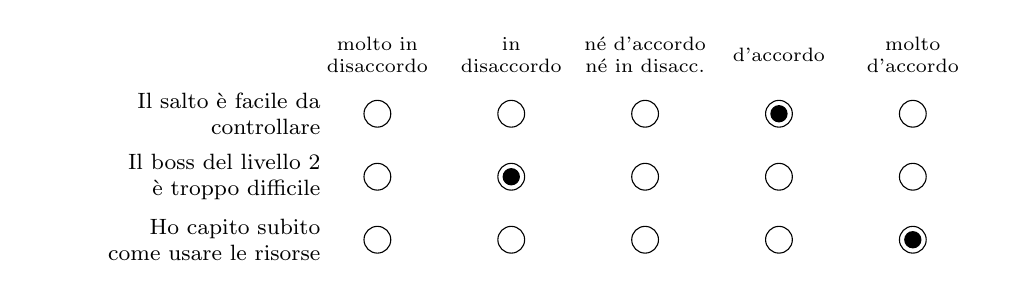
\begin{tikzpicture}[x=1cm, y=1cm,
      gd10lab/.style={font=\footnotesize, anchor=east, text width=3.6cm,
        align=right}]
    % intestazione della scala
    \foreach \i/\t in {1/{molto in\\disaccordo}, 2/{in\\disaccordo},
        3/{né d'accordo\\né in disacc.}, 4/{d'accordo}, 5/{molto\\d'accordo}}
      \node[font=\scriptsize, align=center, text width=1.6cm]
        at (\i*1.7+0.2, 0.75) {\t};
    % righe
    \foreach \y/\q/\s in {0/{Il salto è facile da\\controllare}/4,
        -0.8/{Il boss del livello 2\\è troppo difficile}/2,
        -1.6/{Ho capito subito\\come usare le risorse}/5}{
      \node[gd10lab] at (1.3,\y) {\q};
      \foreach \i in {1,...,5}{
        \draw (\i*1.7+0.2,\y) circle (0.17);
      }
      \fill (\s*1.7+0.2,\y) circle (0.11);
    }
  \end{tikzpicture}
  \caption{Un esempio di domande con scala di Likert a cinque valori (le
  affermazioni sono inventate a scopo illustrativo). Ogni risposta è un
  numero da 1 a 5: si aggrega e si mette in grafico immediatamente.}
  \label{gd10:fig:likert}
\end{figure}

\paragraph{Il ``ma'' delle risposte chiuse.} Ci sono dei ``ma''. Sul
\textbf{genere}, per esempio, o comunque dove si vuole dare al tester ampio
margine di espressione, il docente ``per come è fatto'' spingerebbe per la
risposta libera. Si possono limitare le risposte, come si diceva l'altra
volta (``maschio, femmina, altro, preferisco non rispondere'') senza
risposta libera: ma così \textbf{tutto lo spettro possibile viene mangiato
via}. È un compromesso da fare consapevolmente.

\paragraph{La magnitudine, ma non il perché.} I valori numerici servono a
capire il \textbf{peso percepito} di una meccanica. Se c'è qualcosa di
veramente problematico (i giocatori non hanno capito il level design, o la
progressione è proprio rotta), lo si vede subito: si vede la
\textbf{magnitudine}, se una cosa è piaciuta estremamente o è stata
particolarmente non apprezzata. Ma \textbf{non si sa perché}, e non si sa se
l'utenza ha suggerimenti.

\paragraph{Poi i dati qualitativi.} Qui entrano in gioco i \textbf{dati
qualitativi}: dopo i valori, si chiedono \textbf{maggiori informazioni}. Non
tutti saranno disposti a darle, quindi la domanda può essere
\textbf{facoltativa}; ma \textbf{va fatta}. È quello che il docente chiede
anche agli studenti nei questionari: ``a me non interessa che mi mettiate 1
o 5, mi interessa il perché. Se no non capisco.''

\subsection{Ricompense: meglio le gemme che gli euro}

Il docente mostra esempi di aziende che fanno survey ``estremamente
bene'', tra cui una in cui ha lavorato.\footnote{Il nome dell'azienda nella
trascrizione è illeggibile (``Olio Verso, il mio ex''); non lo si ricostruisce.}
Alcune domande servono già a \textbf{mascherare una categorizzazione
dell'utenza}: aiutano a capire non solo quale elemento è stato percepito
come più importante, ma anche \textbf{che tipo di giocatore} si ha davanti.
``Ma di questo ne parleremo in futuro, mi spiace.''

\paragraph{La ricompensa in gioco.} Il caso migliore di ricompensa, secondo
il docente, è quella \textbf{inclusa nel gioco}: se ne possono generare $N$,
pesa relativamente poco sulla progressione, ed è meglio dare dieci gemme,
dieci \emph{rainbow shards}, ``dieci quello che è'', piuttosto che pagare
100, 500 o 1000 euro in survey. Lo fa anche \emph{Master Duel}, ``visto che
l'abbiamo visto recentemente''.

\paragraph{Il rischio delle risposte a caso.} C'è un rischio: soprattutto nei
survey lunghi, se si dà una ricompensa il giocatore può \textbf{rispondere a
caso} pur di ottenerla. Qui si può approfondire il discorso del
\textbf{margine di errore}: se si vedono risposte particolarmente
\textbf{incoerenti}, o non allineate con il tipo di giocatore che si ha in
mente, si può prendere quella riga e \textbf{non considerarla}.

\paragraph{Approfondimento: survey e interviste secondo Schell.} Nel capitolo
sul playtesting, Schell dà una lista di consigli sui survey che coincide in
buona parte con quella del docente, e la completa:\footnote{Jesse Schell,
\emph{The Art of Game Design}, terza edizione, capitolo 28 (\emph{Good Games
Are Created Through Playtesting}), paragrafo \emph{What Data Will I Collect
after the Play Session?}.} usare \textbf{immagini} quando si chiede di
elementi o scene del gioco, perché il giocatore sappia di che cosa si parla;
preferire agli online \emph{SurveyMonkey} o \emph{Google Forms}, gratuiti o
economici; \textbf{non usare scale da 1 a 10}, ma scale a \textbf{cinque
punti} con ogni punto etichettato (\emph{terribile, abbastanza brutto, così
così, buono, eccellente}), che danno risultati più coerenti; non mettere
troppe domande, o la gente ``si spegne'' verso la fine; dare il survey
\textbf{subito dopo} la sessione; avere qualcuno a disposizione per
chiarimenti; annotare età e genere; e soprattutto \textbf{non prendere i dati
come vangelo}, perché un survey raramente è davvero scientifico e i tester
inventano quando non sono sicuri. Per le domande troppo complesse per un
survey, Schell suggerisce l'\textbf{intervista}, con altri consigli che
rafforzano la lezione: non aspettarsi che i tester siano game designer (non
``il livello 3 sarebbe stato meglio più difficile?'', a cui risponderanno di
no perché i giocatori vogliono sempre il gioco più facile, ma ``ci sono parti
del livello 3 noiose?''); chiedere più di quanto serve (``quali sono le tre
parti che ti sono piaciute meno?'' dà più dati, già ordinati per priorità);
e mettere da parte l'ego, senza difendere il gioco davanti al tester. Il set
di domande che Schell usa nel suo studio, \textbf{FFWWDD}, è un buon
modello per la parte qualitativa:
\begin{enumerate}
  \item qual è stato il momento o l'aspetto più \textbf{frustrante}?
  \item qual è stato il tuo momento o aspetto \textbf{preferito}?
  \item c'era qualcosa che \textbf{volevi} fare e non hai potuto?
  \item se avessi una \textbf{bacchetta magica} (\emph{wand}), che cosa
        cambieresti, aggiungeresti o toglieresti?
  \item che cosa stavi \textbf{facendo}, nell'esperienza (\emph{doing})?
  \item come \textbf{descriveresti} il gioco ad amici e familiari?
\end{enumerate}
L'ordine è voluto: prima si lascia sfogare il tester, poi si cerca il picco
dell'esperienza; le domande 3 e 4 sembrano uguali ma non lo sono (la terza
raccoglie piccoli desideri, la quarta idee fuori dagli schemi); la quinta
rivela l'obiettivo che il giocatore si era dato, la sesta come ha percepito
il senso complessivo dell'esperienza.

% ---------------------------------------------------------------------
\section{Spacchettare i feedback: l'esempio di God of War}
\label{gd10:sec:spacchettare}

\subsection{Due tester}

``Ora facciamo un altro esempio, molto rapido e indolore, presuppongo.'' Si
assume di raccogliere i feedback del \textbf{primo} \emph{God of War}, quello
con Kratos ``incazzato nero'', con le Lame del Caos. I tester sono due,
``chiaramente con nomi fantastici'': \textbf{Bella Isa}, conosciuta anche
come Isabelle (``cuoricino''), e \textbf{Hugh Mikey Jacketman}. Ecco che
cosa dicono (tabella~\ref{gd10:tab:gow-feedback}).

\begin{table}[htbp]
  \centering
  \caption{I feedback dei due tester sul primo \emph{God of War}, come
  presentati a lezione (parafrasati dalla trascrizione).}
  \label{gd10:tab:gow-feedback}
  \small
  \begin{tabular}{@{}p{0.45\textwidth}p{0.45\textwidth}@{}}
    \toprule
    \textbf{Bella Isa} & \textbf{Hugh Mikey Jacketman} \\
    \midrule
    ``Il gioco è estremamente violento: perché dovrei strappare la cassa
      toracica a questo tizio? Non basta ucciderlo?'' &
      ``Fratello, ho impalato Ares e stava agonizzando, piangeva come un
      bambino.'' \\
    \addlinespace
    ``Kratos è un protagonista monodimensionale, che non si evolve mai
      come personaggio.'' &
      ``Kratos è una bestia, mi fa venire voglia di andare in palestra.'' \\
    \addlinespace
    ``È stato divertente battere quel tizio strano con la barba rossa:
      forse era Ade?'' &
      ``Quadrato, quadrato, triangolo: GG, easy mode.'' \\
    \bottomrule
  \end{tabular}
\end{table}

Una volta ricevuti feedback del genere, bisogna farsi delle domande. Il
docente le organizza in quattro passi.

\subsection{Primo: identificare il target audience}

La prima cosa, che la classe ha già inquadrato: \textbf{Isabelle non è il
nostro target audience}, mentre Jacketman probabilmente lo è. Chi dice che
\emph{God of War} è troppo violento, che non vuole strappare la gabbia
toracica a un nemico, va contro tutta la visione del gioco, contro la sua
\emph{action}: è condizione sufficiente per dire che non è il target.

\paragraph{Ma non si ignora.} Questo \textbf{non} significa che abbia senso
ignorare tutto ciò che dice: può aver sollevato punti interessanti. Quindi il
primo punto è \textbf{identificare il target audience}, quanto più possibile.

\subsection{Secondo: la rilevanza statistica}

Il secondo punto è la \textbf{rilevanza statistica}: quanti tester dicono la
stessa cosa?
\begin{itemize}
  \item Se \textbf{sei Isabelle su otto} dicono che Kratos è
        monodimensionale, è \textbf{accettabilissimo}. Il docente non pensa
        (``qui qualcuno potrebbe smentirlo'') che l'obiettivo narrativo del
        primo \emph{God of War} fosse creare un personaggio con cui fare
        \emph{bonding}, o che si evolvesse nel tempo. Lo sarebbe per il
        \emph{God of War} del 2018,\footnote{Nella trascrizione ``God of
        War 2019''; il capitolo con Atreus, di cui si sono visti i pilastri
        (sezione~\ref{gd9:sec:pilastri}), è uscito nel 2018.} e lì sarebbe
        un problema. Qui, il fatto che un pubblico non in target lo abbia
        notato è positivo: è \textbf{proprio l'obiettivo}.
  \item Se \textbf{due Jacketman} dicono ``quadrato, quadrato, triangolo: GG
        easy mode'', anche questo è esattamente ciò che si voleva. Quella
        era la \textbf{combo base} su cui è stato \textbf{bilanciato} il
        gioco, in modo che lo si potesse finire usando solo quella: la combo
        più semplice dell'universo rendeva il gioco completabile anche da
        persone con \textbf{bassa abilità reattiva}. Se lo dice un numero
        ridotto di persone, va bene: era pensata per essere così.
\end{itemize}

\subsection{Terzo: tradurre il linguaggio}

Bisogna anche \textbf{tradurre} ciò che dice l'utenza, perché si potrebbe non
condividerne il linguaggio, il gergo, lo slang.
\begin{itemize}
  \item ``Il tizio strano con la barba rossa'': chi era? Isabelle dice Ade,
        ma \textbf{non è Ade}: non c'è un Ade con la barba rossa nel primo
        \emph{God of War}; è Ares. Bisogna capire che cosa intende. E una
        volta capito, allora sì che c'è un problema: \textbf{non ha
        compreso chi fosse} quel personaggio, né che rilevanza avesse nella
        storia.
  \item ``Kratos è una bestia'': è positivo? Il docente dice di sì; ma
        potrebbe intendere qualcos'altro. Lo stesso vale per ``GG easy
        mode'': non è scontato che un designer sappia che cosa significa
        \emph{good game, easy}, né è fondamentale.
\end{itemize}

\paragraph{Chiedete.} Più si va avanti con l'età, più probabilmente non si
condividerà un certo slang con i giovani. Non serve aprire un dizionario, o
andare per strada come nel meme del signore attempato che si veste da
ragazzo e va in giro con lo skateboard.\footnote{Il docente lo chiama ``il
meme di Burns''; il meme descritto è quasi certamente quello di Steve
Buscemi in \emph{30 Rock} (``\emph{How do you do, fellow kids?}'').} Il
tester ce l'avete davanti: \textbf{chiedeteglielo}.

\subsection{Quarto: le risposte emotive}

L'ultimo punto sono le \textbf{risposte emotive}, cioè \emph{come} il tester
dice le cose.
\begin{itemize}
  \item Se Isabelle si lamenta della violenza \textbf{ed è triste}, va bene:
        non è il target. Ma se lo dice con un sorriso a trentadue denti,
        si potrebbe aver colto comunque il punto: potrebbe essere, a livello
        viscerale, proprio l'effetto che si cerca nel gameplay.
  \item ``\emph{It was fun}'', come si sa
        (sezione~\ref{rv:t1:sec:linguaggio}), \textbf{non significa
        nulla}: bisogna capire quale emozione Isabelle associa a quel
        divertimento nello sconfiggere il ``\emph{red beard guy}''. Potrebbe
        essere la \textbf{challenge}, o addirittura il \textbf{fiero} (era
        un ostacolo particolarmente difficile, e batterlo le ha dato
        piacere); potrebbe essere l'aver \textbf{masterato la combo} nel
        batterlo; o l'aver \textbf{punito il male}, più sul lato narrativo
        che meccanico. O si sa esattamente chi si ha davanti, e allora si sa
        da dove deriva il suo divertimento (anche qui con un margine di
        errore); oppure, più semplicemente, \textbf{glielo si chiede}.
  \item Jacketman che racconta in modo esagitato di aver impalato Ares e di
        aver goduto del suo pianto è \textbf{positivo}: con \emph{God of War}
        il target vuole distruggere gli dèi, ``strappargli le braccia, le
        palpebre e qualsiasi cosa sia legata al loro corpo''. Non è solo ciò
        che si desidera, è la \textbf{reazione emotiva} che si cerca
        nell'utenza.
  \item E il fatto che, dopo aver giocato, corra in palestra a fare panca
        piana? ``Probabilmente sì'', è positivo: probabilmente è proprio ciò
        che si vorrebbe.
\end{itemize}

\paragraph{Un processo da cui non si sfugge.} La
figura~\ref{gd10:fig:spacchettare} riassume il processo. ``Questo è un
processo che dovete fare: non si sfugge.''

\begin{figure}[htbp]
  \centering
  \begin{tikzpicture}[
      gd10box/.style={draw, rounded corners=2pt, align=center,
        text width=3.4cm, minimum height=1.35cm, font=\footnotesize},
      gd10arr/.style={-{Stealth[length=2.2mm]}, thick},
      node distance=0.45cm]
    \node[gd10box, fill=gray!8] (fb) {\textbf{Feedback}\\ grezzo del
      tester};
    \node[gd10box, right=of fb] (t1) {\textbf{1. Target?}\\ è nel target
      audience? (non si ignora comunque)};
    \node[gd10box, right=of t1] (t2) {\textbf{2. Quanti?}\\ rilevanza
      statistica sul totale};
    \node[gd10box, below=0.9cm of t2] (t3) {\textbf{3. Che cosa intende?}\\
      tradurre slang e gergo};
    \node[gd10box, left=of t3] (t4) {\textbf{4. Come lo dice?}\\ risposta
      emotiva; quale emozione dietro il ``fun''};
    \node[gd10box, left=of t4, fill=gray!20] (pb) {\textbf{Problema}\\
      (non soluzione), da confrontare con la vision};
    \draw[gd10arr] (fb) -- (t1);
    \draw[gd10arr] (t1) -- (t2);
    \draw[gd10arr] (t2) -- (t3);
    \draw[gd10arr] (t3) -- (t4);
    \draw[gd10arr] (t4) -- (pb);
    \node[font=\scriptsize, align=center, text width=7cm] at
      ($(t3.south)!0.5!(t4.south)+(0,-0.55)$) {nel dubbio, a ogni passo:
      \textbf{chiedete al tester}};
  \end{tikzpicture}
  \caption{I quattro passi per spacchettare un feedback dell'utenza, come
  emergono dall'esempio di \emph{God of War} (ricostruzione schematica).}
  \label{gd10:fig:spacchettare}
\end{figure}

% ---------------------------------------------------------------------
\section{I feedback dei competitor}
\label{gd10:sec:competitor}

I feedback si possono prendere anche \textbf{sui competitor}, e non solo dai
propri test: dai canali \textbf{Twitch}, \textbf{YouTube}, ``quello che
volete''. Lì si vedono subito le cose particolarmente \textbf{memorabili}, o
che l'utenza ricorda con \textbf{nostalgia} o piacere. Anche queste vanno
spacchettate.

\paragraph{I commenti su YouTube.} Il docente mostra alcuni commenti su
\emph{God of War}.
\begin{itemize}
  \item Un utente scrive che l'\textbf{Idra} era il suo boss preferito, con
        cinque risposte e 97 like: magari è un'opinione condivisa.
        \emph{God of War} va ridimensionato, ``perché è enorme''; ma
        potrebbe valere la pena capire \textbf{perché} l'Idra era il boss
        preferito, ed eventualmente riprodurre quel sistema, o quella boss
        fight, in un'altra forma e in un'altra veste in un nuovo gioco. Una
        ``mostra bestiale'', e così via.
  \item Un altro scrive che un certo attacco ``\emph{will always be
        legendary}'':\footnote{Nella trascrizione ``The Light Attack'' e
        ``pseudo life attack''; l'attacco specifico citato nel commento non
        è ricostruibile con certezza.} bisogna capire perché, e magari
        prevedere una meccanica o un sistema di combo che lo includa.
  \item Un terzo apprezza il Kratos nuovo, cresciuto, che ha imparato dai
        propri errori e sviluppa un senso di paternità verso il figlio.
        Funziona, e non solo perché è uno dei punti dominanti del gioco:
        anche perché \textbf{l'utenza è cresciuta}. Gli adolescenti che
        giocavano ai primi \emph{God of War} ora sono adulti che giocano al
        nuovo, e si rivedono in quel Kratos con dei rimpianti: rileggono il
        personaggio anche attraverso la propria crescita.
\end{itemize}

\paragraph{Le recensioni su Steam.} ``Prendetelo ovunque'', anche su
\textbf{Steam} (si è visto anche \emph{Steam 250}). Anche qui si spacchetta:
quanti prodotti ha il recensore, che giocatore è, \textbf{quante ore} ha
giocato, se ha avuto il gioco in \textbf{early access} o no, se l'ha ricevuto
gratuitamente. I dati di Steam di solito mostrano queste cose. Il docente
assume che si prendano feedback da giochi di cui non si ha il controllo, e
quindi senza i profili che tracciano tutto ciò che l'utenza fa: si cerca di
prendere ciò che dicono e di \textbf{estrapolarne le emozioni o le
motivazioni principali}, anche con l'aiuto di Quantic Foundry
(sezione~\ref{sec:quantic-foundry}).

\paragraph{Non sempre aiutano.} Certe recensioni aiutano poco: ``\emph{Spooky
scary game}'' dice forse che il recensore cercava l'horror, qualche emozione
trainante dell'horror, e che ama le battute. Ci sono recensori peculiari
che recensiscono tutti i giochi nello stesso modo, ``è l'internet''. E un
commento come ``\emph{next game: God of War 5}'' fa presumere che il
recensore voglia un quinto capitolo, ma non se ne ha la certezza.

% ---------------------------------------------------------------------
\section{La curva dell'utenza e i consigli finali}
\label{gd10:sec:gaussiana}

\subsection{Evangelisti e odiatori}

Come ultimi \emph{tips and tricks}, si assume che tutta l'utenza (anzi, tutti
i giocatori) si possa disporre su una \textbf{gaussiana}, una curva normale o
``curva a campana''. Come si diceva tempo addietro
(sezione~\ref{sec:analisi-utenti}), ai due estremi ci sono le persone che
amano alla follia il gioco, gli \textbf{evangelisti}, che lo consigliano
agli altri, e i suoi profondi \textbf{odiatori}. Sono persone di cui
\textbf{non è necessario modificare la traiettoria}.
\begin{itemize}
  \item Gli \textbf{evangelisti} non sono del tutto ignorabili: a loro si
        possono chiedere feedback, si può chiedere se le cose piacciono,
        soprattutto molto prima che escano. Ma avranno la loro linea di
        pensiero e difficilmente la cambieranno: ``dovete veramente
        distruggere l'anima del gioco per fargli cambiare idea''.
  \item Gli \textbf{odiatori} difficilmente ameranno il gioco, perché
        \textbf{non sono il target}: sono molto lontani dalle motivazioni
        che il gioco può far scaturire.
\end{itemize}

\paragraph{Il formaggio.} Al docente non piacciono la pizza con il formaggio
sciolto né i latticini in generale: ``questo non significa che Parmareggio
debba preoccuparsi di cambiare il gusto per farmelo mangiare per forza''.
Non è parte di quel discorso. Allo stesso modo, un giocatore che non giocherà
mai un PvP estremo, o un gioco di zombie, non va convertito.

\paragraph{Gli estremi sono i più vocali.} Questi due estremi sono molto
spesso \textbf{quelli che si fanno sentire di più}: c'è sempre chi si lamenta
del bilanciamento, e di solito sono le persone che \textbf{giocano di più in
assoluto}, e che hanno l'abitudine di mandare feedback e scrivere commenti.
Quando si cercano feedback ci sono spesso questi \emph{bias}. Anche se ci si
riconosce in un giocatore che si lamenta, non è detto che sia da ascoltare:
il target effettivo potrebbe non essere quello, ``anche se vi piace tanto il
gioco''.

\paragraph{La rabbia attiva.} C'è poi uno \textbf{sbilanciamento} tra i due
estremi: generalmente si fanno sentire di più gli \textbf{odiatori}. Perché
\textbf{la rabbia è un'emozione attivante}: porta le persone ad agire, a
muoversi, a fare cose. La felicità, la pace dei sensi, portano invece a uno
stato di calma: si vuole restare lì, ``in ammollo'', in quella beatitudine.
Bisogna quindi badare bene a chi sta scrivendo: l'estremo negativo sarà
sempre molto vocale. Se, fatti i conti, il feedback negativo è una
percentuale minima del totale, la community è sana: ``un 5\% di community
incazzata va bene'', poi dipende dalla community.

\paragraph{Approfondimento: gli evangelisti secondo Bateman e Boon.} Anche
\emph{21st Century Game Design} osserva che i giocatori più orientati alla
sfida sono ``l'\emph{hardcore} vocale'', che ama discutere di giochi online,
e che molti giochi raggiungono il pubblico \emph{casual} proprio passando per
questi gruppi di \textbf{evangelisti}. Ma, aggiunge il libro, la facilità di
gioco che il pubblico casual desidera è ``anatema'' per l'esperienza di
sfida, dominata dal fiero, che gli evangelisti cercano.\footnote{Chris
Bateman, Richard Boon, \emph{21st Century Game Design}, 2005, capitolo 3,
paragrafi sui cluster \emph{Hardcore} e \emph{Casual}.} È un esempio
concreto del perché il feedback dell'estremo più vocale non coincide con
quello del grosso dell'utenza.

\subsection{Problemi, mai soluzioni}

Secondo consiglio: \textbf{usate i feedback dei giocatori per identificare i
problemi, mai le soluzioni}. Il giocatore può proporre una soluzione, magari
anche attuabile, ma deve passare per una vostra ``estrema valutazione
cauta''. Si prende il feedback per \textbf{mostrare i problemi}; non si sale
mai a bordo delle soluzioni dell'utenza. Vale per i giocatori, e
\textbf{al limite} anche per le persone esperte a cui si chiede un feedback.

\subsection{Difendete la vostra visione}

Terzo consiglio, che sembra andare contro alcune cose dette: \textbf{difendete
la vostra visione}. Se si è fatto il design esattamente come si è detto, con
la ricerca fatta ``precisa, a modino'', e si è sicuri delle decisioni di
design e della loro implementazione, alla fine dei conti \textbf{i
professionisti siete voi}. La scelta di modificare o meno, di togliere o
meno qualcosa, passa per voi. Bisogna considerare il target audience e i
suoi gusti; ma magari una cosa \textbf{la odia perché non l'ha compresa}, o
perché c'è un altro problema, e non è detto che sia sbagliata di base,
soprattutto se le meccaniche sono allineate con la visione. Assunto che si
sia fatto tutto (ricerca dell'audience, lavoro per il suo bene),
\textbf{l'ultima parola resta vostra}.

\paragraph{Anche nel team.} Vale forse meno con i giocatori e di più
\textbf{all'interno del team}, se le responsabilità sono divise e le
meccaniche sono date ai designer. Se gli artisti dicono ``no, non ci
piace'', la cosa è relativa, con due premesse: che il gioco sia
\textbf{design first}, e che ciò che si è identificato come meccanica di
sistema sia da implementare. Gli artisti la \textbf{vestono}. Diverso è il
caso in cui si è pensato a un livello che cambia l'arte ogni due secondi, e
l'artista chiede ``ce la facciamo?'': quello è un altro discorso, di
fattibilità.

\subsection{Data informed, non data driven}

Quarto consiglio, conseguenza del secondo: \textbf{\emph{data informed
design}, not \emph{data driven}}. Tutti i dati che si raccolgono, anche dai
competitor, devono \textbf{aiutare a identificare un problema}, non dare già
la soluzione. La slide dice ``\emph{unless specified}'': alcuni giochi,
generalmente i \textbf{game as a service}, i \emph{live game} come
\emph{Candy Crush}, o i giochi di Supercell,\footnote{Nella trascrizione ``i
giochi super sell''; quasi certamente Supercell, lo studio di \emph{Clash of
Clans} e \emph{Clash Royale}.} sono in gran parte \emph{data driven}, per
massimizzare l'utenza e per facilità. Ma è un caso legato ai game as a
service, non ai molti casi di cui si parla nelle lezioni. ``Ricordate sempre
che il design è \textbf{50\% scienza e 50\% arte}.''

\subsection{Non eliminate subito ciò che l'utenza odia}

Ultimo consiglio: se l'utenza odia qualcosa (una meccanica, un personaggio),
\textbf{non eliminatelo subito}. Non si salta sulla soluzione appena arriva
un feedback, non si corre immediatamente ai ripari: ci si ferma, si
spacchetta il feedback, si fa un passo indietro.

\paragraph{La Control Room.} È un problema di molte persone, e il docente lo
lamentava anche con Alessandro. Il caso tipico, nei progetti annuali
dell'accademia: arriva la \textbf{Control Room}, ``la grande tavola rotonda
delle persone che dovete temere'', e dice ``questa meccanica non funziona,
me la cambiate?''. Non si prende e si corre a sistemare tutto perché il capo,
o chi sta sopra di lui, ha detto di farlo. Ci si ferma e si cerca di capire
che cosa è stato detto: magari il feedback è legato a qualcosa che non
avevano, o la meccanica non è stata capita, o il problema deriva da
un'altra parte. Se poi, dopo averci riflettuto e averne parlato con lo
\textbf{stakeholder} (sezione~\ref{sec:stakeholder}), il modus operandi resta
quello indicato, va bene, è accettabile. Ma non si crea il panico: spesso
queste reazioni portano a \textbf{problemi a cascata}. E magari ciò che la
playerbase odia era già stato previsto: un altro designer ci aveva già
pensato e lo aveva documentato. Ci si prende il tempo per
\textbf{affrontare il feedback, tradurlo, e poi risolverlo}.

\subsection{Prima e dopo il lancio}

L'ultima slide è un'approssimazione di un caso ideale: il design perfetto,
prima del lancio, con l'utenza disposta su una curva normale
(figura~\ref{gd10:fig:gaussiana}).
\begin{itemize}
  \item Agli estremi, circa il \textbf{3\%} per parte: quelli che amano il
        gioco alla follia e quelli che lo odiano ``alla morte'', ``quelli
        che vi mandano le minacce'' e sono ``il core della vostra
        tossicità''. Non interessano.
  \item Poi circa il \textbf{13\%} a cui il gioco piace molto, e il
        \textbf{13\%} a cui non piace: non verranno sotto casa con i forconi
        di notte, ma il gioco non fa per loro.
  \item Al centro le due fasce che \textbf{interessano di più}: la fascia
        \textbf{neutra positiva} e quella \textbf{neutra negativa}. Sono le
        persone che \textbf{oscillano} tra il voler e il non voler giocare il
        gioco, tra il comprarlo e il non comprarlo.
\end{itemize}

\begin{figure}[htbp]
  \centering
  \begin{tikzpicture}[x=1.55cm, y=4.2cm]
    % fasce
    \fill[gray!45] (-4,0) -- plot[domain=-4:-2, samples=30]
      (\x,{exp(-\x*\x/2)}) -- (-2,0) -- cycle;
    \fill[gray!25] (-2,0) -- plot[domain=-2:-1, samples=30]
      (\x,{exp(-\x*\x/2)}) -- (-1,0) -- cycle;
    \fill[gray!10] (-1,0) -- plot[domain=-1:0, samples=30]
      (\x,{exp(-\x*\x/2)}) -- (0,0) -- cycle;
    \fill[gray!10] (0,0) -- plot[domain=0:1, samples=30]
      (\x,{exp(-\x*\x/2)}) -- (1,0) -- cycle;
    \fill[gray!25] (1,0) -- plot[domain=1:2, samples=30]
      (\x,{exp(-\x*\x/2)}) -- (2,0) -- cycle;
    \fill[gray!45] (2,0) -- plot[domain=2:4, samples=30]
      (\x,{exp(-\x*\x/2)}) -- (4,0) -- cycle;
    % curva e assi
    \draw[thick] plot[domain=-4:4, samples=80] (\x,{exp(-\x*\x/2)});
    \draw[-{Stealth[length=2mm]}] (-4.3,0) -- (4.5,0);
    \foreach \x in {-2,-1,0,1,2} \draw[dashed, gray] (\x,0) --
      (\x,{exp(-\x*\x/2)});
    % percentuali
    \node[font=\scriptsize] at (-2.75,0.06) {$\sim$3\%};
    \node[font=\scriptsize] at (-1.5,0.1) {13\%};
    \node[font=\scriptsize] at (-0.5,0.35) {34\%};
    \node[font=\scriptsize] at (0.5,0.35) {34\%};
    \node[font=\scriptsize] at (1.5,0.1) {13\%};
    \node[font=\scriptsize] at (2.75,0.06) {$\sim$3\%};
    % etichette
    \node[font=\scriptsize, align=center, anchor=north] at (-3,-0.02)
      {odiatori\\(``tossicità'')};
    \node[font=\scriptsize, align=center, anchor=north] at (-1.5,-0.02)
      {non gli\\piace};
    \node[font=\scriptsize, align=center, anchor=north] at (-0.5,-0.02)
      {neutri\\negativi};
    \node[font=\scriptsize, align=center, anchor=north] at (0.5,-0.02)
      {neutri\\positivi};
    \node[font=\scriptsize, align=center, anchor=north] at (1.5,-0.02)
      {gli\\piace};
    \node[font=\scriptsize, align=center, anchor=north] at (3,-0.02)
      {evangelisti};
    \draw[thick] (-1,1.07) -- (1,1.07);
    \draw[thick] (-1,1.03) -- (-1,1.07); \draw[thick] (1,1.03) -- (1,1.07);
    \node[above=2pt, font=\scriptsize, align=center] at (0,1.07)
      {le fasce che oscillano: \textbf{qui} si gioca la conversione};
  \end{tikzpicture}
  \caption{L'utenza disposta su una curva normale, prima del lancio, come
  approssimata a lezione. Le percentuali corrispondono a quelle di una
  distribuzione normale (circa 34\% entro una deviazione standard dalla
  media per parte, 13,6\% tra una e due, 2,1\% oltre le due, arrotondato a
  lezione al 3\%).}
  \label{gd10:fig:gaussiana}
\end{figure}

\paragraph{Dopo il lancio: la conversione.} Dopo il lancio, idealmente
(``non è che funziona sempre così''), si deve aver \textbf{spostato la
curva}: gli odiatori restano odiatori, ma una parte di chi era negativo
diventa neutro, e la fascia neutra positiva diventa quella che \textbf{ha
comprato il gioco e lo gioca}.\footnote{La descrizione della slide
post-lancio, nella trascrizione, è frammentaria (``questa faccia rimane
rosso; questa scala diventa neutrale; e questa parte qui è ok, funziona''):
il senso generale, uno spostamento delle fasce centrali verso il positivo,
è chiaro; il dettaglio di ciascuna fascia no.} Cercare di attuare questa
\textbf{conversione} è spesso il motivo per cui si fanno i \textbf{DLC}, il
contenuto post-lancio, le \emph{patch}: al di là del bug fixing, il
contenuto post-lancio serve esattamente a convertire questa parte
dell'utenza. È il caso migliore possibile, ma è un'approssimazione da tenere
a mente quando si rilascia un gioco e quando si legge l'utenza.

% ---------------------------------------------------------------------
\section{Una lezione jolly}
\label{gd10:sec:jolly}

``Domande? Ok.'' La lezione sui feedback è finita ``con ampio margine di
anticipo''. Il docente carica le slide (``non l'ho fatto prima, ahimè''; ma
gli studenti hanno comunque la registrazione, e quando la rivedranno
``sarete troppo \emph{deep}'' perché importi) e decide di usare il tempo
rimasto. Invece di andare avanti con il programma, si fa un altro
\emph{deep dive} su documentazione e \emph{pitching}: ``lezione extra,
chiamala così, una jolly: ce la giochiamo adesso''.

\paragraph{Le due lezioni più importanti dell'anno.} Prima, un avviso: nel
mese ci sono ancora due lezioni, e gli studenti devono cercare di essere
presenti a entrambe, perché tratteranno \textbf{gli argomenti più importanti
dell'anno}. Sono due:
\begin{itemize}
  \item la \textbf{profilazione dell'utenza} e gli \textbf{archetipi di
        giocatori};
  \item il \textbf{``framework principe''}: uno dei più noti, ``non
        necessariamente il più funzionale'', ma estremamente
        \textbf{malleabile}, da cui ne sono nati molti altri; un
        \textbf{benchmark} per l'analisi e il design strutturato dei
        giochi.\footnote{Il docente non lo nomina. La descrizione (il più
        noto, malleabile, capostipite di molti altri framework di analisi)
        fa pensare all'MDA (\emph{Mechanics, Dynamics, Aesthetics}) di
        Hunicke, LeBlanc e Zubek; ma è un'ipotesi.}
\end{itemize}

\paragraph{Due documenti senza forma netta.} Visto che si è parlato di
playtest, si vedono due documenti specifici del mondo del design: il
\textbf{versioning tracker} (o \emph{versioning document}, ``come vogliate
chiamarlo'') e il \textbf{documento di playtest}, che accoglie i dati dei
playtest. Il docente avverte subito che \textbf{nessuno dei due ha una forma
netta}: dirà che esistono, a che cosa servono e come si fanno
indicativamente, ma la forma ``sta un po' a voi, e anche a me''.
\begin{itemize}
  \item Il documento di playtest dipende molto non solo dal progetto, ma da
        \textbf{che cosa si vuole far testare}: qual è l'obiettivo del
        playtest, che cosa si va a cercare.
  \item Il versioning è ``un concetto un po' spinoso'': serve non solo ai
        designer ma soprattutto ai \textbf{producer}, e può espandersi o
        contrarsi a seconda che riguardi l'intero progetto, un grosso
        sistema o una singola meccanica. Per questo spesso non è un
        documento a sé, ma \textbf{una parte del documento di design}, del
        processo di design che gli studenti hanno iniziato con l'ultimo
        task: il versioning dovrebbe \textbf{chiudere} quel documento.
\end{itemize}

% ---------------------------------------------------------------------
\section{Il versioning tracker}
\label{gd10:sec:versioning}

\subsection{Il libretto di istruzioni dell'IKEA}

La sezione si apre con un meme di \emph{The Office} (``che io aborro
profondamente, però sappiatelo''). L'obiettivo di un documento di
tracciamento è \textbf{tracciare la produzione}: avere delle \textbf{linee
guida}. ``È come il libretto di istruzioni dell'IKEA'': il designer crea una
linea guida proiettata nel futuro che, se seguita, porta alla
\textbf{versione corretta} della feature, del progetto, di qualsiasi cosa.

\paragraph{Spesso assorbito in altri documenti.} Questa linea guida dipende
così tanto dalla feature e dal progetto che, nella stragrande maggioranza dei
casi, \textbf{viene assorbita} e diventa una parte di altri documenti: di
design, di meccaniche, di sistemi, ma anche di livelli. È un tracker, ``un
\emph{doc}, come volete chiamarlo'', che generalmente è un
\textbf{paragrafo specifico del GDD o dell'LDD}. Vale per molti documenti:
più si andrà avanti, più si avranno conoscenza, esperienza e libertà nel
combinare elementi, separarli, prendere un pezzo di un framework e unirlo a
un altro. ``Come sempre, valutate la migliore situazione possibile da
momento a momento. Questo è importantissimo.''

\subsection{Le regole d'oro}

\begin{description}
  \item[Notificate il producer] Se esiste un documento di tracking, lo si
        dice \textbf{sempre} al producer: dove sta e a che cosa serve.
  \item[Aggiornatelo] Soprattutto, \textbf{se lo si inserisce, va
        aggiornato}, ``e questo ce lo dimentichiamo sempre'': a che punto
        della versione siamo, che cosa è stato fatto, che cosa no, che cosa
        manca.
  \item[Chiamate in causa gli altri dipartimenti] Una feature include il
        lavoro di molti dipartimenti: il \textbf{sound} (il sound designer),
        i \textbf{VFX} (il VFX artist), le \textbf{animazioni} e il
        \textbf{rigging}, la \textbf{3D art} per un modello, e così via. Un
        tracker fatto bene chiama in causa i task di tutti. Se non si sa
        qualcosa, per esempio quanto tempo serve per un modello o un
        rig, e anche solo ``vi solletica il cervello un leggero dubbio'',
        \textbf{lo si chiede sempre}: ``o mai lo saprete, ragazzi''.
\end{description}

\subsection{Che cosa contiene}

Il docente mostra un esempio creato \emph{ad hoc}, perché tutti quelli che ha
sono sotto NDA; e, ``che culo'', è proprio un paragrafo specifico, fatto su
Miro. L'\textbf{obiettivo} è il \textbf{controllo}: tenere traccia di tutte
le versioni necessarie di una feature, dal punto in cui c'è un
\textbf{prototipo giocabile e testabile} fino alla \textbf{versione completa
nel core}, di solito la \textbf{1.0}.

\paragraph{La 1.0 è l'MVP.} La 1.0 è il cosiddetto \textbf{MVP},
\emph{Minimum Viable Product} (o \emph{Project}): la versione minima,
``vestita'' con i feedback necessari per essere \textbf{implementabile} nel
gioco, nella sua versione 1. Si può andare oltre (un bilanciamento di fino,
feedback addizionali), ma questa timeline proiettata nel futuro va scritta, e
serve a capire \textbf{dove si è} lungo di essa.

\paragraph{Gli elementi.} Servono:
\begin{enumerate}
  \item i diversi \textbf{stadi} (\emph{stage}) della feature;
  \item i \textbf{sottotask} inclusi in ciascuno stadio;
  \item il \textbf{tempo} e le \textbf{risorse} allocati per ciascuno stadio
        (responsabilità soprattutto del producer);
  \item i \textbf{check} che ciascuno stadio deve passare per saltare al
        successivo;
  \item le \textbf{dipendenze} (\emph{dependencies}): la relazione tra task
        e sottotask. Al documento di design o di analisi del designer può
        corrispondere, per l'artista, il \emph{blockout} di una mesh o di
        un'animazione; va spiegato \textbf{quale dipartimento} lo fa e
        \textbf{in quale stadio} è necessario farlo, considerando il tempo a
        disposizione.
\end{enumerate}

\paragraph{Funzione maggiore di forma.} Deve essere \textbf{essenziale} da
leggere: tutti lo leggono, quindi nessuno ha voglia di leggerlo, ed è spesso
una lista immensa. Per ogni sottotask basta il \textbf{dipartimento} (``magari
con un colorino associato, sarebbe carino''), lo \textbf{stadio} o lo
\textbf{status}, e la \textbf{descrizione} del task. ``Molto di più non
serve.''

\paragraph{Accessibile.} Tutti devono potervi accedere. L'utilità di un
documento di versioning a sé è proprio che i non designer (artisti,
programmatori), interessati solo a sapere quali task devono fare, vanno lì
senza doversi leggere il documento di design. D'altra parte, avere una serie
di version document sparsi può essere \textbf{dispersivo}: ci si assicura che
tutti, e soprattutto i producer, possano accedervi; e come indirizzare le
persone nel posto giusto dipende dal \textbf{compendium}
(sezione~\ref{gd9:sec:compendium}) o dal producer stesso.

\paragraph{Da qui a Jira.} Un'altra cosa che si fa spesso è prendere le
descrizioni dal tracker e riportarle su un \textbf{sistema di tracciamento}
come \textbf{Jira} o \textbf{Asana}, quello che si usa, che il producer
adopera per tracciare il progresso di tutto il gioco e assegnare i task di
settimana in settimana. Ciò che è nel tracker è \textbf{uno a uno} con ciò che
il producer comunica al team: è come un calendario delle cose da fare, per
chi non è avvezzo a girare tra i documenti. ``E ci sta, assolutamente.''

\paragraph{Mantenimento.} Come detto, è estremamente importante: i designer,
o in generale gli \textbf{owner} della feature, lo modificano e lo tengono
\textbf{aggiornato}; a ogni aggiornamento, i membri del team rilevanti per
quella feature, sistema o progetto vanno \textbf{notificati}.

\subsection{L'esempio: la camminata}

L'esempio mostrato riguarda il \textbf{sistema di camminata e di locomozione
base}, con un \emph{disclaimer}: non è omnicomprensivo, ci sarebbero molte
altre voci da includere, e andrebbe spiegata la legenda. La
tabella~\ref{gd10:tab:versioning} lo ricostruisce.

\begin{table}[htbp]
  \centering
  \caption{Ricostruzione dell'esempio di versioning della camminata mostrato
  a lezione. Le versioni intermedie, i tempi e alcune voci sono indicativi;
  nell'esempio originale alcune celle erano lasciate a ``TBD'' per
  semplicità, cosa che in un documento vero non si fa.}
  \label{gd10:tab:versioning}
  \footnotesize
  \begin{tabular}{@{}p{0.07\textwidth}p{0.14\textwidth}p{0.37\textwidth}p{0.08\textwidth}p{0.24\textwidth}@{}}
    \toprule
    \textbf{Ver.} & \textbf{Dipartimento} & \textbf{Task} &
      \textbf{Tempo} & \textbf{Check per avanzare} \\
    \midrule
    0.1 & Level design & creare la \emph{gym} di test & 1 h &
      bug check; test a livello di team; approvazione del lead di ogni
      dipartimento coinvolto \\
        & Programmazione & premendo D il personaggio cammina verso destra
      a velocità 10 & & \\
        & Game design & testare l'azione di camminata nella gym & & \\
    \addlinespace
    0.5 & Programmazione & sistema di accelerazione che modifica la
      velocità & \ldots & come sopra \\
        & Game design & \emph{tuning} della velocità & & \\
    \addlinespace
    1.0 & Animazione, VFX, SFX & animazioni di camminata, effetti visivi e
      sonori; eventuali restrizioni artistiche & \ldots & come sopra:
      la feature è pronta per essere inserita e \emph{shippata} (MVP) \\
    \addlinespace
    $>$1.0 & \ldots & bilanciamento fine, feedback aggiuntivi (1.5,
      2.0\ldots) & \ldots & \ldots \\
    \bottomrule
  \end{tabular}
\end{table}

\paragraph{La 1.0 è accettabile.} Si assume che, arrivati alla 1.0, la
feature sia buona da inserire nel gioco: la si può \textbf{accettare}. È
sempre migliorabile, quindi ci potrebbero essere una 1.5, una 2 e così via,
da spiegare. E non si lasciano celle \textbf{TBD} (``io l'ho messo per
semplicità, ma non è che lo lasciate''): alla 1 la feature è generalmente
accettabile per essere messa nel progetto e \emph{shippata}.

\paragraph{Un riassunto del documento di design.} Il tracker \textbf{riassume}
ciò che il documento di design spiega nel dettaglio. Per esempio, molte delle
descrizioni scritte dagli studenti nei task avrebbero potuto benissimo stare
qui, asciutte; ma avrebbero avuto bisogno di molta più spiegazione e
profondità altrove, cioè nel documento di design.

\paragraph{I check di produzione.} Per ciascuno stadio: \textbf{bug check},
\textbf{testing a livello di team} e \textbf{approvazione dei lead} di
ciascun dipartimento coinvolto. Il \textbf{lead di programmazione} dà
un'occhiata al codice, si assicura che la \textbf{nomenclatura} sia usata
correttamente e che non siano state fatte ``spaghettate di codice''
all'interno del progetto. Il \textbf{lead di design} si preoccupa che il
\textbf{GDD} sia allineato, e che la visione del design sia esattamente
quella allineata con l'idea.

\paragraph{Più avanti nelle versioni.} Alla 0.5 si \textbf{tuna la
velocità}: il programmatore deve creare un sistema di accelerazione che
modifica la velocità, con i suoi check. Per la 1.0 potrebbero servire
\textbf{restrizioni artistiche} che prima non erano necessarie; nell'esempio
mancano le \textbf{animazioni}, che vanno considerate, e i \textbf{VFX} e gli
\textbf{SFX}. ``Ripeto, non è omnicomprensivo: guardatelo sempre in maniera
molto più intima.''

\paragraph{Approfondimento: dire che cosa si consegna, e quando.} Il
versioning è la versione documentale di una delle chiavi di comunicazione di
Schell viste sopra (sezione~\ref{gd10:sec:pillole}): la \textbf{chiarezza}
come impegno concreto e specifico. ``Faccio il combattimento entro giovedì''
lascia la porta spalancata ai malintesi; ``tre o cinque pagine
sull'interfaccia del combattimento a turni entro giovedì alle 17'' no. Un
tracker con stadi, sottotask, dipartimenti, tempi e check è esattamente una
lista di impegni del secondo tipo.

% ---------------------------------------------------------------------
\section{Il documento di playtest}
\label{gd10:sec:playtest-doc}

\subsection{Obiettivo: ottenere dati}

``Ok, passiamo al documento di playtest, anche perché questo è l'ultimo.''
L'esempio mostrato tratta alcuni punti molto utili. L'obiettivo di un
documento di playtest è \textbf{ottenere dati dal playtest}: ``non molto di
più, non molto di meno''.

\paragraph{Perché è difficile codificarlo.} Dipende da \textbf{che cosa si
va a testare}.
\begin{itemize}
  \item Se si dà un \textbf{prototipo} in mano a un \textbf{esperto} (e non
        a un utente), all'esperto si fanno alcune domande, ma non c'è tutto
        il gioco: si prendono \textbf{dati specifici} e si fanno
        \textbf{domande specifiche}.
  \item Se si ha \textbf{l'intero gioco}, il survey sarà fatto in un altro
        modo.
  \item Se è un \textbf{gioco fisico}, il documento viene messo in mano a
        qualcuno che lo riempie a ogni sessione di playtest, annotando che
        cosa è cambiato, che cosa è stato diverso, \textbf{chi ha vinto},
        \textbf{quanto tempo} è durata la partita, \textbf{quanti giocatori}
        erano al tavolo, e così via (lo si è visto nel corso di analog game
        design, capitolo~\ref{a12:cap:playtest}).
  \item Per un progetto \textbf{digitale} la questione è diversa: lo
        spettro è estremamente ampio.
\end{itemize}

\subsection{I punti fermi}

Alcune cose, però, si possono dire con precisione
(tabella~\ref{gd10:tab:playtest}).

\begin{description}
  \item[Un bacino di dati] Il documento serve a \textbf{ottenere e
        controllare} feedback e dati: è un bacino di dati specifici
        dell'utenza.
  \item[Collegato al GDD] Può essere unito a un \textbf{GDD}: se si fa il
        playtest di una specifica feature, il documento di playtest può
        essere collegato al GDD di quella feature, per vedere, versione per
        versione, quali feedback si sono ottenuti, che cosa è andato bene e
        che cosa male nella \textbf{0.3}, che cosa è cambiato nella
        \textbf{0.5}, e così via. È il punto d'incontro con il versioning.
  \item[Centrato sul test] È centrato su \textbf{che cosa deve essere
        testato} e su che cosa deve ricevere particolare attenzione da chi
        testa.
  \item[Che cosa contiene] Che cosa è stato testato; \textbf{come} i tester
        sono stati testati o osservati, cioè quali erano i riferimenti
        principali: ci interessava che fossero \textbf{spaventati} (un
        horror)? Che fossero in \textbf{tensione}? Che fossero
        \textbf{soddisfatti del bilanciamento} generale (un \emph{economy
        test})? E di quali \textbf{tool} sono stati dotati i tester.
  \item[Forma] Finché è circoscritto al team di design, per la
        documentazione interna: \textbf{funzione maggiore di forma}. Per
        qualsiasi cosa destinata a tester e giocatori esterni al team
        (``generica persona che passa per strada, le dai il PC in mano e ti
        gioca il gioco''): \textbf{funzione maggiore o uguale a forma}. In
        quel caso, se ha la forma di un survey, va reso minimamente
        \textbf{esteticamente appagante}.
  \item[Accesso] Solo i team legati alla feature e alle sessioni di
        playtest devono potervi accedere. ``Gli altri non ci interessano.''
  \item[Responsabilità] I \textbf{designer} lo modificano. A volte il
        \textbf{lead} dà linee guida; ma generalmente, se si testa una
        feature, è il designer che l'ha fatta a creare il documento di
        playtest.
\end{description}

\paragraph{I tool dei QA.} Il punto sui tool merita un esempio. Internamente,
se c'è un dipartimento di \textbf{QA}, i tester sono provvisti di sistemi di
\textbf{debug}, magari di \emph{cheat} di \textbf{invincibilità} perché devono
saltare delle parti, magari dell'intero gioco a disposizione. In un
\textbf{open world} in cui interessa testare il bioma Y e non il bioma X, e
si parte da molto lontano, si può fornire un sistema di
\textbf{teletrasporto} e di invincibilità: tutte cose centrate a migliorare
l'esperienza su \textbf{ciò che deve essere testato}, non su tutto il resto.
Ma queste cose vanno \textbf{documentate}, e soprattutto sono i tester a
dirlo quando danno il feedback: ``ho testato il gioco con questi settaggi, ho
fatto queste cose, è successo questo, questo e questo''.

\begin{table}[htbp]
  \centering
  \caption{Uno schema possibile di documento di playtest, ricostruito dai
  punti visti a lezione (non è il template del docente).}
  \label{gd10:tab:playtest}
  \small
  \begin{tabular}{@{}p{0.27\textwidth}p{0.65\textwidth}@{}}
    \toprule
    \textbf{Voce} & \textbf{Esempio} \\
    \midrule
    Feature e versione & camminata, v0.5 (link al GDD della feature) \\
    Obiettivo del test & la velocità e l'accelerazione risultano
      controllabili? \\
    Che cosa osservare & frustrazione nei salti di precisione; tempo per
      attraversare la gym \\
    Tester & numero, tipo di giocatore, target sì/no \\
    Setup e tool & build, settaggi, cheat (invincibilità, teletrasporto) \\
    Dati quantitativi & tempi, morti, valori Likert del survey \\
    Dati qualitativi & risposte aperte, note di osservazione, citazioni \\
    Rispetto alla versione precedente & che cosa è cambiato, che cosa è
      migliorato o peggiorato \\
    Problemi individuati & elenco, con priorità (problemi, non soluzioni) \\
    \bottomrule
  \end{tabular}
\end{table}

\subsection{Il documento non basta: bisogna testare}

``Lo ripetiamo adesso'': è importante che il gioco venga testato. Il
documento di playtest serve come \textbf{cartina tornasole}, come metro di
misura di ciò che succede; ma bisogna \textbf{farlo giocare}, altrimenti è
inutile fare questo tipo di documenti. Prima il gioco viene testato, meglio
è, perché prima si arriva a una versione migliore, sapendo che cosa non
funziona. ``Facciamola girare più velocemente possibile, questa ruota, e
mettiamola in moto il prima possibile'' (figura~\ref{gd10:fig:ruota}).

\paragraph{Nessun task.} Su questi due documenti non c'è un task. Ma bisogna
ricordarsi che \textbf{esistono}, e il discorso su quanto possano essere
legati o slegati da altri documenti, \textbf{in entrambi i casi
principalmente il GDD}. ``Questa è la cosa più importante.''

\paragraph{Approfondimento: la lente del playtesting.} Schell distingue
quattro tipi di test che spesso si confondono:\footnote{Jesse Schell,
\emph{The Art of Game Design}, terza edizione, capitolo 28, e lente \#103,
\emph{The Lens of Playtesting}.} i \textbf{focus group} (interviste a
potenziali giocatori su ciò che piace o no, utili soprattutto per decidere la
priorità relativa di feature ben definite, ma con una cattiva fama perché
spesso condotti male); il \textbf{QA testing} (che non ha nulla a che fare
con quanto il gioco sia piacevole: cerca bug); lo \textbf{usability testing}
(se interfaccia e sistemi sono intuitivi); e il \textbf{playtesting} vero e
proprio, cioè vedere se il gioco produce l'esperienza per cui è stato
progettato. La sua lente riassume ciò che un documento di playtest deve
saper dire prima ancora del test: \emph{perché} facciamo questo playtest?
\emph{Chi} deve esserci? \emph{Quando} testiamo? \emph{Dove}? \emph{Che
cosa} cerchiamo? \emph{Come} otterremo le informazioni che ci servono? E,
aggiunge Schell, la domanda ``il mio gioco è divertente?'' non basta: le
domande devono essere il più specifiche possibile (``i giocatori capiscono
come si gioca?'', ``il livello 3 è troppo lungo?'', ``ci sono strategie
dominanti?''). Schell confessa anche di \textbf{odiare} il playtest, per
paura che il gioco non piaccia; ed è proprio il motivo per cui bisogna farlo
presto e spesso.

% ---------------------------------------------------------------------
\section{La chiusura: lavorare entro dei limiti}
\label{gd10:sec:chiusura}

\subsection{Che cosa è arrivato della documentazione pratica?}

Avanza ancora un po' di tempo, e il docente chiede se ci sono questioni da
aprire. L'unica cosa che ritiene utile vedere, nel poco tempo rimasto, è il
riscontro sul discorso della \textbf{documentazione pratica} fatto con
l'esercizio sui core elements (sezione~\ref{gd9:sec:riformattazione}):
``quanto è stato recepito, solo voi me lo potete dire''.

\paragraph{Le risposte della classe.} Una studentessa risponde che le ha
mostrato dei \textbf{trucchi} utilizzabili di base, e le ha fatto capire in
che cosa deve migliorare (nella trascrizione, non del tutto chiara, renderlo ``più credibile'').
``Questa è metà della partita'', commenta il docente, ``perché poi c'è tutta
la parte di creazione del documento.'' Altri citano il \textbf{titolo}
trattato come titolo della scheda (perché effettivamente è più grande), il
\textbf{modo di sfruttare gli spazi} (``una cosa che sto imparando piano
piano''), la distinzione tra gli spazi e le \textbf{linee}. ``Molto bene.''

\paragraph{Un modo, non l'unico.} Ciò che si è visto non è l'unico modo, è
\textbf{un} modo, e con solo alcuni strumenti. Ma il punto è
\textbf{sfruttare in modo creativo le poche cose a disposizione}: i
documenti Google non offrono chissà quante possibilità, ed è anche utile
\textbf{lavorare entro certi limiti}.

\subsection{La soluzione sta nel problema}

``Filosoficamente'' è ciò che tocca fare nel trovare soluzioni: prendere
qualcosa che si ha sotto mano e che si usa nel modo previsto (prevedibile),
e provare a vederlo da un altro punto di vista; cercare soluzioni con il poco
che si ha, ma usato in modo \textbf{creativo e innovativo}. Spesso la
soluzione di un problema \textbf{sta già nel modo in cui il problema è
formulato}. Lo si vedrà più avanti con altri tipi di documentazione: c'è
proprio una filosofia di design legata a \textbf{quanto è grande un
documento}, a quanto farlo diventare enorme o quanto stringerlo. Per quanto
possa piacere o no la documentazione, ragionare entro questi limiti
costringe a formulare il problema in modo diverso, e formulandolo in modo
diverso si trova qualcosa a cui non si era pensato.

\paragraph{Con due lire.} ``Sapete quante volte mi scervellavo su una
soluzione con sistemi difficili da implementare, tecnologie complesse o
design particolarmente stravaganti, quando invece la soluzione si poteva
fare con veramente due lire, due spicci?'' Non va dimenticato.

\subsection{I blocchetti di Lego}

``Ragionate per immagini. Quando possibile, \textbf{mostrate}.'' E
soprattutto iniziate a pensare a come gli elementi visti finora possono
\textbf{comporsi l'uno con l'altro}. Il \textbf{flowchart}
(sezione~\ref{sec:flowchart-usi}): dove potrebbe essere inserito, in quale
condizione, se si sta facendo design o se si deve prevedere che cosa
aspettarsi dall'utenza? La \textbf{Theory of Planned Behavior} vista
l'ultima volta (sezione~\ref{gd9:sec:tpb}):\footnote{Nella trascrizione
``questo qui aterior plan''.} un domani potrebbe servire a documentare un
sistema, o ancora meglio la \textbf{strategia} che il giocatore adotta e
\textbf{perché} la adotta. Sono cose estremamente importanti, che diventano
necessarie in futuro. ``Iniziate a farlo ora, perché poi ve lo imporrò di
più'': unire questi blocchi, ``questi blocchettini di Lego che vi do''.

\subsection{I prossimi appuntamenti}

Si chiude con leggero anticipo. La lezione successiva non è il lunedì
seguente: ci si rivede il \textbf{20}, poi il \textbf{27} (``da calendario,
che avete tutti''). A dicembre ci sono due lezioni, una con il docente e una
con Diego. E per chi ha recuperato la registrazione fin qui: ``di solito si
dice tipo scrivete `zucca', e so che siete arrivati fin qui; ma io non posso
leggere i vostri commenti, quindi\ldots''.

% ---------------------------------------------------------------------
\section*{Punti chiave del capitolo}
\addcontentsline{toc}{section}{Punti chiave del capitolo}

\begin{itemize}
  \item Nel task su \emph{Metroid Dread} il compendium resta quasi vuoto, ma
        va diviso per dipartimenti principali, con status e legenda; la
        vision contiene pilastri, prime emotions e moods, must do, must not,
        nice to have e USP, \textbf{sempre tre}. I pilastri qui si estraggono
        \emph{a posteriori} dal gameplay. Se il docente dice ``poi vi do il
        task'', ricordateglielo.
  \item Una \textbf{legenda della formattazione} serve se ci sono acronimi,
        status o molti strumenti; l'obiettivo è non renderla necessaria. È
        utile soprattutto nei documenti di bilanciamento.
  \item Fare design significa \textbf{trattare tutti i dettagli}: numeri
        indicativi, casi limite (che succede quando il battle pass finisce?),
        nuove UI e nuove parole chiave spiegate. Test: con questo documento
        potrei implementare il sistema? Se non lo scrivete, i programmatori
        fanno di testa loro, e la responsabilità è vostra.
  \item La severità dei feedback non è mai personale ed è in funzione della
        crescita; il mondo là fuori non sempre dà feedback costruttivi.
  \item Assunti di base: dall'altra parte c'è un \textbf{umano};
        le \textbf{soft skill} sono la prima discriminante per essere assunti
        o licenziati; i feedback sono \textbf{costruttivi}. Feedback 101:
        precisi e rispettosi, empatici, e coltivare queste capacità.
  \item Un feedback è \textbf{costruttivo} (preciso, chiaro, analitico),
        \textbf{neutrale} (dice anche ciò che funziona, e perché, in uno
        stato emotivo neutro), \textbf{sincero} (tra adulti e professionisti),
        \textbf{risolutivo} (una soluzione suggerita, non imposta) e
        \textbf{senza giudizio}. La \textbf{tecnica del sandwich non
        funziona}: meglio una lista chiara.
  \item \textbf{Chiari}: riformulare finché entrambi sono soddisfatti.
        \textbf{Precisi}: reference esatte, guardarle insieme, dare tempo.
        \textbf{Analitici}: obiettivo e intenzione di ciò che si valuta,
        allineamento con la vision, dati, percezione del target.
  \item Non state zitti nei meeting (effetto valanga); un team, non una
        famiglia: fallimenti condivisi, successi festeggiati, meriti
        riconosciuti. Il \textbf{framing} è potentissimo (Starbucks, i nove
        dentisti su dieci). Linguaggio del corpo neutro, o si rimanda.
  \item Il \textbf{fiero} nasce da una sfida molto al di sopra delle skill
        attuali, superata dopo tempo, fallimenti e tentativi; è un picco, va
        trattato con i guanti, ed è un gancio potentissimo (\emph{Dark
        Souls}, \emph{Hollow Knight}).
  \item Raccogliere: \textbf{testare presto} (anche i documenti), test di
        validazione all'inizio ed economy test con il QA; \textbf{chiedere}
        chi sono i tester per pesarne i feedback; \textbf{collezionare} più
        dati possibili, registrando.
  \item Survey: \textbf{sotto i cinque minuti} (dichiarati), poca agency,
        \textbf{scala di Likert} per la magnitudine, poi una domanda
        qualitativa (anche facoltativa) per il perché; linguaggio semplice;
        ricompense in gioco meglio che in denaro, scartando le risposte
        incoerenti.
  \item Spacchettare un feedback: \textbf{target} sì o no (ma non si
        ignora), \textbf{rilevanza statistica}, \textbf{tradurre} il gergo,
        leggere la \textbf{risposta emotiva}; nel dubbio, chiedere.
  \item L'utenza sta su una gaussiana: \textbf{evangelisti e odiatori} sono
        i più vocali (la rabbia attiva), ma le fasce che contano sono quelle
        \textbf{neutre}, da convertire anche con DLC e contenuti post-lancio.
  \item Feedback per i \textbf{problemi, mai per le soluzioni};
        \textbf{difendete la visione}; \emph{data informed}, non \emph{data
        driven} (salvo i game as a service); non eliminate subito ciò che
        l'utenza odia: fermatevi e spacchettate.
  \item Il \textbf{versioning tracker} è il libretto IKEA della feature,
        spesso un paragrafo del GDD: stadi, sottotask, tempo e risorse,
        check, dipendenze, fino alla 1.0 (\textbf{MVP}); essenziale,
        accessibile, aggiornato, notificato al producer.
  \item Il \textbf{documento di playtest} serve a ottenere dati: che cosa si
        testa, come si osserva, con quali tool; collegabile al GDD versione
        per versione; funzione $>$ forma internamente, $\geq$ verso
        l'esterno. Ma senza far giocare il gioco non serve a nulla.
  \item Lavorare entro dei limiti costringe a riformulare i problemi: la
        soluzione spesso sta nel problema, e si fa con due lire. Iniziate a
        comporre i blocchetti (flowchart, TPB, documenti).
\end{itemize}
